\section{Ricerca di fisica Beyond Standard Model con i VAEs}
\label{fisica_BSM_VAEs}

In quest'ultimo capitolo verrà presentata una possibile applicazione dei Variational Autoencoders nel campo della fisica delle alte energie, con lo scopo di ricercare segnali di nuova fisica BSM, cioè oltre il Modello Standard. \\
Gli esperimenti portati avanti al \textit{Large Hadron Collider} hanno l'obiettivo di esplorare la fisica spingendosi sempre a più alte energie; attualmente, nonostante la scoperta del bosone di Higgs abbia confermato la validità dello SM, questo modello non riesce a dare alcune risposte a domande aperte nel campo della fisica delle alte energie, quali lo \textbf{Hierarchy problem} e l'origine della materia oscura. \\
Nella ricerca di nuova fisica possono essere portati avanti due approcci, detti \textit{model dependent} e \textit{model independent}. Nel primo caso la ricerca di nuova fisica avviene con un particolare modello in mente, così che è possibile creare un algoritmo di ricerca ottimizzato per il modello target. D'altra parte questo approccio fa si che si focalizzi solo su un particolare canale di ricerca, e quindi manchi di generalità. Dall'altro lato una ricerca model independent ha il pregio di non essere legata ad una particolare teoria fisica e quindi è capace di ricercare eventuali segnali di nuova fisica senza fare alcuna ipotesi sulla loro natura, o la loro origine. Come descritto nel capitolo \ref{ML: metodi e caratteristiche} quest'ultimo approccio ha molte analogie con il modo in cui i metodi di ML non supervisionati classificano i dati.\\
Nel caso descritto il VAE verrà addestrato su dati SM simulati, in modo da fare un modello del fondo. L'approccio seguito sarà model dependent: infatti la ricerca sarà ottimizzata per un processo supersimmetrico di produzione elettrodebole di una coppia chargino/neutralino (partner fermionici dei bosoni elettrodeboli). In questo canale il chargino decadrà [descrivi il processo]. \\
Se l'addestramento si dovesse rivelare efficace, e la sensibilità al processo a cui si è interessati fosse buona, il processo verrà ripetuto utilizzando i dati dell'esperimento, per cercare di osservare l'anomalia direttamente nel campione di dati raccolti. \\
Questo ulteriore passaggio è possibile solo in virtù dell'approccio \textit{Unsupervised} per cui non è necessario dare all'algoritmo le etichette fondo/segnale durante la fase di addestramento. Per lo stesso motivo si capisce perché un algoritmo \textit{Supervised} non possa essere in generale direttamente applicato ai dati sperimentali; infatti questa seconda categoria di modelli richiede nella fase di addestramento le etichette fondo/segnale per ciascun evento fisico al fine di impararne la distinzione. Si deve perciò ricorrere necessariamente alle simulazioni MC con tutte le incertezze modellistiche annesse. 

\color{red}
approfondire il discorso model dependent/independent \\
descrivi il processo ... cosa devo mettere ? \\
\color{black}

\newpage

%%%%%%%%%%%%%%%%%%%%%%%%%%%%%%%%%%%%%%%%%%%%%%%%%%%%%%%%%%%%%%%%

\subsection{Dataset}
\label{dataset}
Per l'addestramento del modello e per la successiva fase di verifica sono stati utilizzati i dati prodotti attraverso simulazioni Montecarlo (MC), in base alla teoria di riferimento (SUSY). Le variabili fisiche che verranno utilizzate per descrivere ogni evento sono otto ($\textit{met}$, $\textit{mt}$, $\textit{mbb}$, $\textit{mct2}$, $\textit{mlb1}$, $\textit{lep1Pt}$, $\textit{njet30}$, $\textit{nBjet30-MV2c10}$) e sono le stesse utilizzate nell'analisi fisica relativa allo studio \cite{susy_alberto}. Di conseguenza lo spazio iniziale, che dovrà essere compresso dal VAE, sarà 8-dimensionale. \\
Attraverso la simulazione MC vengono prodotti eventi sia di background che di segnale.\\ 
Prima di passare alla fase di codifica, gli eventi (sia di segnale che di background) sono stati sottoposti ad una serie di tagli di preselezione sulle variabili, come riportato nella tabella~\ref{tab:tagli di preselezione}.

\begin{table}[h!]
	\centering
	\begin{tabular}{lc}
		\hline
		&Preselezione \\
		\hline
		Esattamente un leptone di segnale&Vero\\
		met\ trigger&Vero\\
		$2-3$ jets con $p_{T}>30 GeV$&Vero\\
		$b$-tagged jet&[1-3]\\
		met\ &$> 220$ GeV\\
		mt\ &$> 50$ GeV\\
		mbb\ &[$100-140$]GeV\\
		mct\ &$>100$GeV\\
		\hline
	\end{tabular}
	\caption{Sono riportati i tagli di preselezione applicati sia agli eventi di segnale che di background, prodotti attraverso una simulazione MC.}
	\label{tab:tagli di preselezione}
\end{table} 
Gli eventi prodotti con il metodo MC sono stati divisi, come si richiede in un processo di apprendimento automatico, in una training data set, un validation data set ed un test data set. Successivamente, per rendere coerente la selezione del segnale simulando una raccolta dati con le attuali capacità e specifiche del LHC, gli eventi di validation e test sono stati ripesati per ottenere la giusta luminosità.\\
Per ottenere i nuovi pesi $w_{j}^{'}$ a partire da quelli validi prima dello split $w_{j}$, è stata usata la seguente formula ~\cite{HiggsChalllenge}:

\begin{equation}
	\label{eq:ripesaggio}
    w_j^{'}=  w_{j}\frac{\sum_{i} w_{i} \textbf{1} \lbrace y_{i}=fondo\rbrace }{\sum_{i\in S^{'}}w_{i} \textbf{1} \lbrace y_{i}=fondo\rbrace }  
\end{equation}

Dove $y_{i}$ è l'etichetta (segnale o fondo) dello i-esimo evento e \textbf{1} è la funzione indicatrice (\textbf{1} {$y_{i}$ = il fondo} è zero per un evento di segnale e pari ad uno per un evento di fondo).

\color{red}
qui è da chiedere per tutte le correzioni
\color{black}

\newpage

%%%%%%%%%%%%%%%%%%%%%%%%%%%%%%%%%%%%%%%%%%%%%%%%%%%%%%%%%%%%%%%%

\subsection{Architettura del modello}
\label{architettura del modello}
Per quanto riguarda la struttura del VAE si specifica che il numero di neuroni negli strati nascosti è pari a cinquanta e che la dimensione dello spazio latente è pari a tre; inoltre la funzione di attivazione dei neuroni è la ReLU, cioè una funzione definita nel seguente modo:
\begin{equation}
	f(x) = \max(0,x)
\end{equation} 
Parlando invece del processo di apprendimento, sono state impostate 2000 epoche, cioè tutti i dati vengono riproposti all'algoritmo per duemila volte; inoltre la \textit{Loss Function} utilizzate è quella standard, composta da un termine legato all'errore di ricostruzione ed uno relativo alla \textit{KL divergency} (moltiplicato per un fattore $\beta=0.6$). Per il processo di discesa del gradiente è stato impostato inizialmente un \textit{learning rate} pari a 0.003, con una diminuzione del 20\% ogni qualvolta il modello non migliora per venti epoche consecutive; inoltre è stata impostata una \textit{batch size} pari a 200, quindi l'aggiornamento dei pesi della rete avviene dopo aver cumulato l'errore su 200 eventi di training. Infine si sottolinea che il processo di addestramento termina o perché si è arrivati alle 2000 epoche o perché la \textit{Validation Loss} non migliora per 50 epoche consecutive.\\
Il modello è stato sviluppato in Python usando le librerie Keras (tensorflow backend).


\subsection{Addestramento del VAE}
\label{simulazione}
Il VAE deve essere addestrato in modo tale da rilevare eventuali indizi di fisica BSM come delle anomalie, cercando di dimostrarsi sensibile ad una ampia gamma di possibili segnali.\\
Un classificatore binario, ovvero un modello capace di discriminare fra due sole categorie (segnale e background), viene addestrato su un training data set i cui eventi di segnale sono generati facendo riferimento ad un determinato modello; tuttavia quando ne verranno presentati altri prodotti con diversi modelli, allora la classificazione risulterà totalmente arbitraria ed è qui che si evince il limite principale di una ricerca model dependent. Un ulteriore vantaggio del VAE ed in generale degli approcci model independent, rispetto a quelli model dependent, è quello di poter essere applicato direttamente sui dati come anticipato nella sezione introduttiva di questo capito (\ref{fisica_BSM_VAEs}). In questo modo si evitano quei problemi di incertezze modellistiche legate alle simulazioni montecarlo.\\
In linea con ciò che è già stato illustrato nel capitolo \ref{VAEs}, gli eventi di segnale e di background, che sono stati prodotti attraverso simulazioni MC, sono rappresentabili in uno spazio 8-dimensionale. Durante il processo di addestramento del VAE gli eventi di background vengono compressi nello spazio latente (tridimensionale), decompressi per essere ricostruiti e poi confrontati con quelli iniziali per il calcolo dell'errore e quindi per dare il via al processo di backpropagation (\ref{reti neurali}). \\
Dopo la fase di addestramento si verifica che il VAE abbia imparato come ricostruire gli eventi fisici di background usati per l'addestramento, dopo averli compressi nello spazio latente. A tal proposito vengono confrontate le distribuzioni originali date in input con quelle rigenerate dalla rete. Allo stesso tempo, si ci aspetta che il modello  commetta un errore di ricostruzione maggiore quando, invece che eventi di background, vengono dati in input eventi di segnale. La limitata capacità di generalizzare su questa nuova categoria di eventi mai visti durante la procedura di addestramento dovrebbe indurre il VAE ad una ricostruzione meno accurata. Come si vedrà è possibile allora usare la distribuzione dell'errore di ricostruzione per eventi di background e segnale per discriminare tra queste due tipologie di eventi.\\
Tra i contributi originali di questa tesi vi è anche la possibilità di pesare in maniera diversa il contributo che le diverse variabili fisiche che definiscono un evento possono apportare al processo di discriminazione e, per questo motivo, verranno presentati due casi: nel primo le otto variabili avranno tutte lo stesso peso, mentre nel secondo si proverà a capire se, dando maggiore importanza ad alcune di esse, si otterrà un processo di discriminazione più efficiente. E' infatti possibile che il VAE, concentrandosi su di una variabile più significativa per la ricostruzione del background ma non altrettanto per il segnale, possa sfruttare questa differenza per aumentare la forbice di errore di ricostruzione tra background e segnale. Rimane a questo punto da capire quali delle variabili possano aiutare in questo compito. Le possibilità sono almeno due: da un lato si possono sfruttare conoscenze o intuizioni teoriche riguardo il potere discriminante di alcune delle variabili, mentre dall'altro si può procedere in maniera brute-force(\ref{iperparametri e grid search}) sulle possibili configurazioni dei pesi da dare alle diverse variabili.\\

\color{red}
qui mi ha lasciato il VAE come approccio model independet
\color{black}

\newpage

%%%%%%%%%%%%%%%%%%%%%%%%%%%%%%%%%%%%%%%%%%%%%%%%%%%%%%%%%%%%%%%%

\subsection{Risultati}
\label{risultati}

\subsubsection{Processo di rigenerazione degli eventi}
\label{rigenerazione_eventi}
Come primo passo bisogna capire se, a seguito del processo di addestramento, il VAE è in grado di ricostruire gli eventi di background in maniera ottimale. Il risultato del processo di ricostruzione è riportato in figura~\ref{ricostruzione}, dove vengono confrontate le distribuzioni dei dati in input (punti blu) con quelle ricostruite dal VAE (punti rossi). 
\begin{figure}[h!]
	\centering
	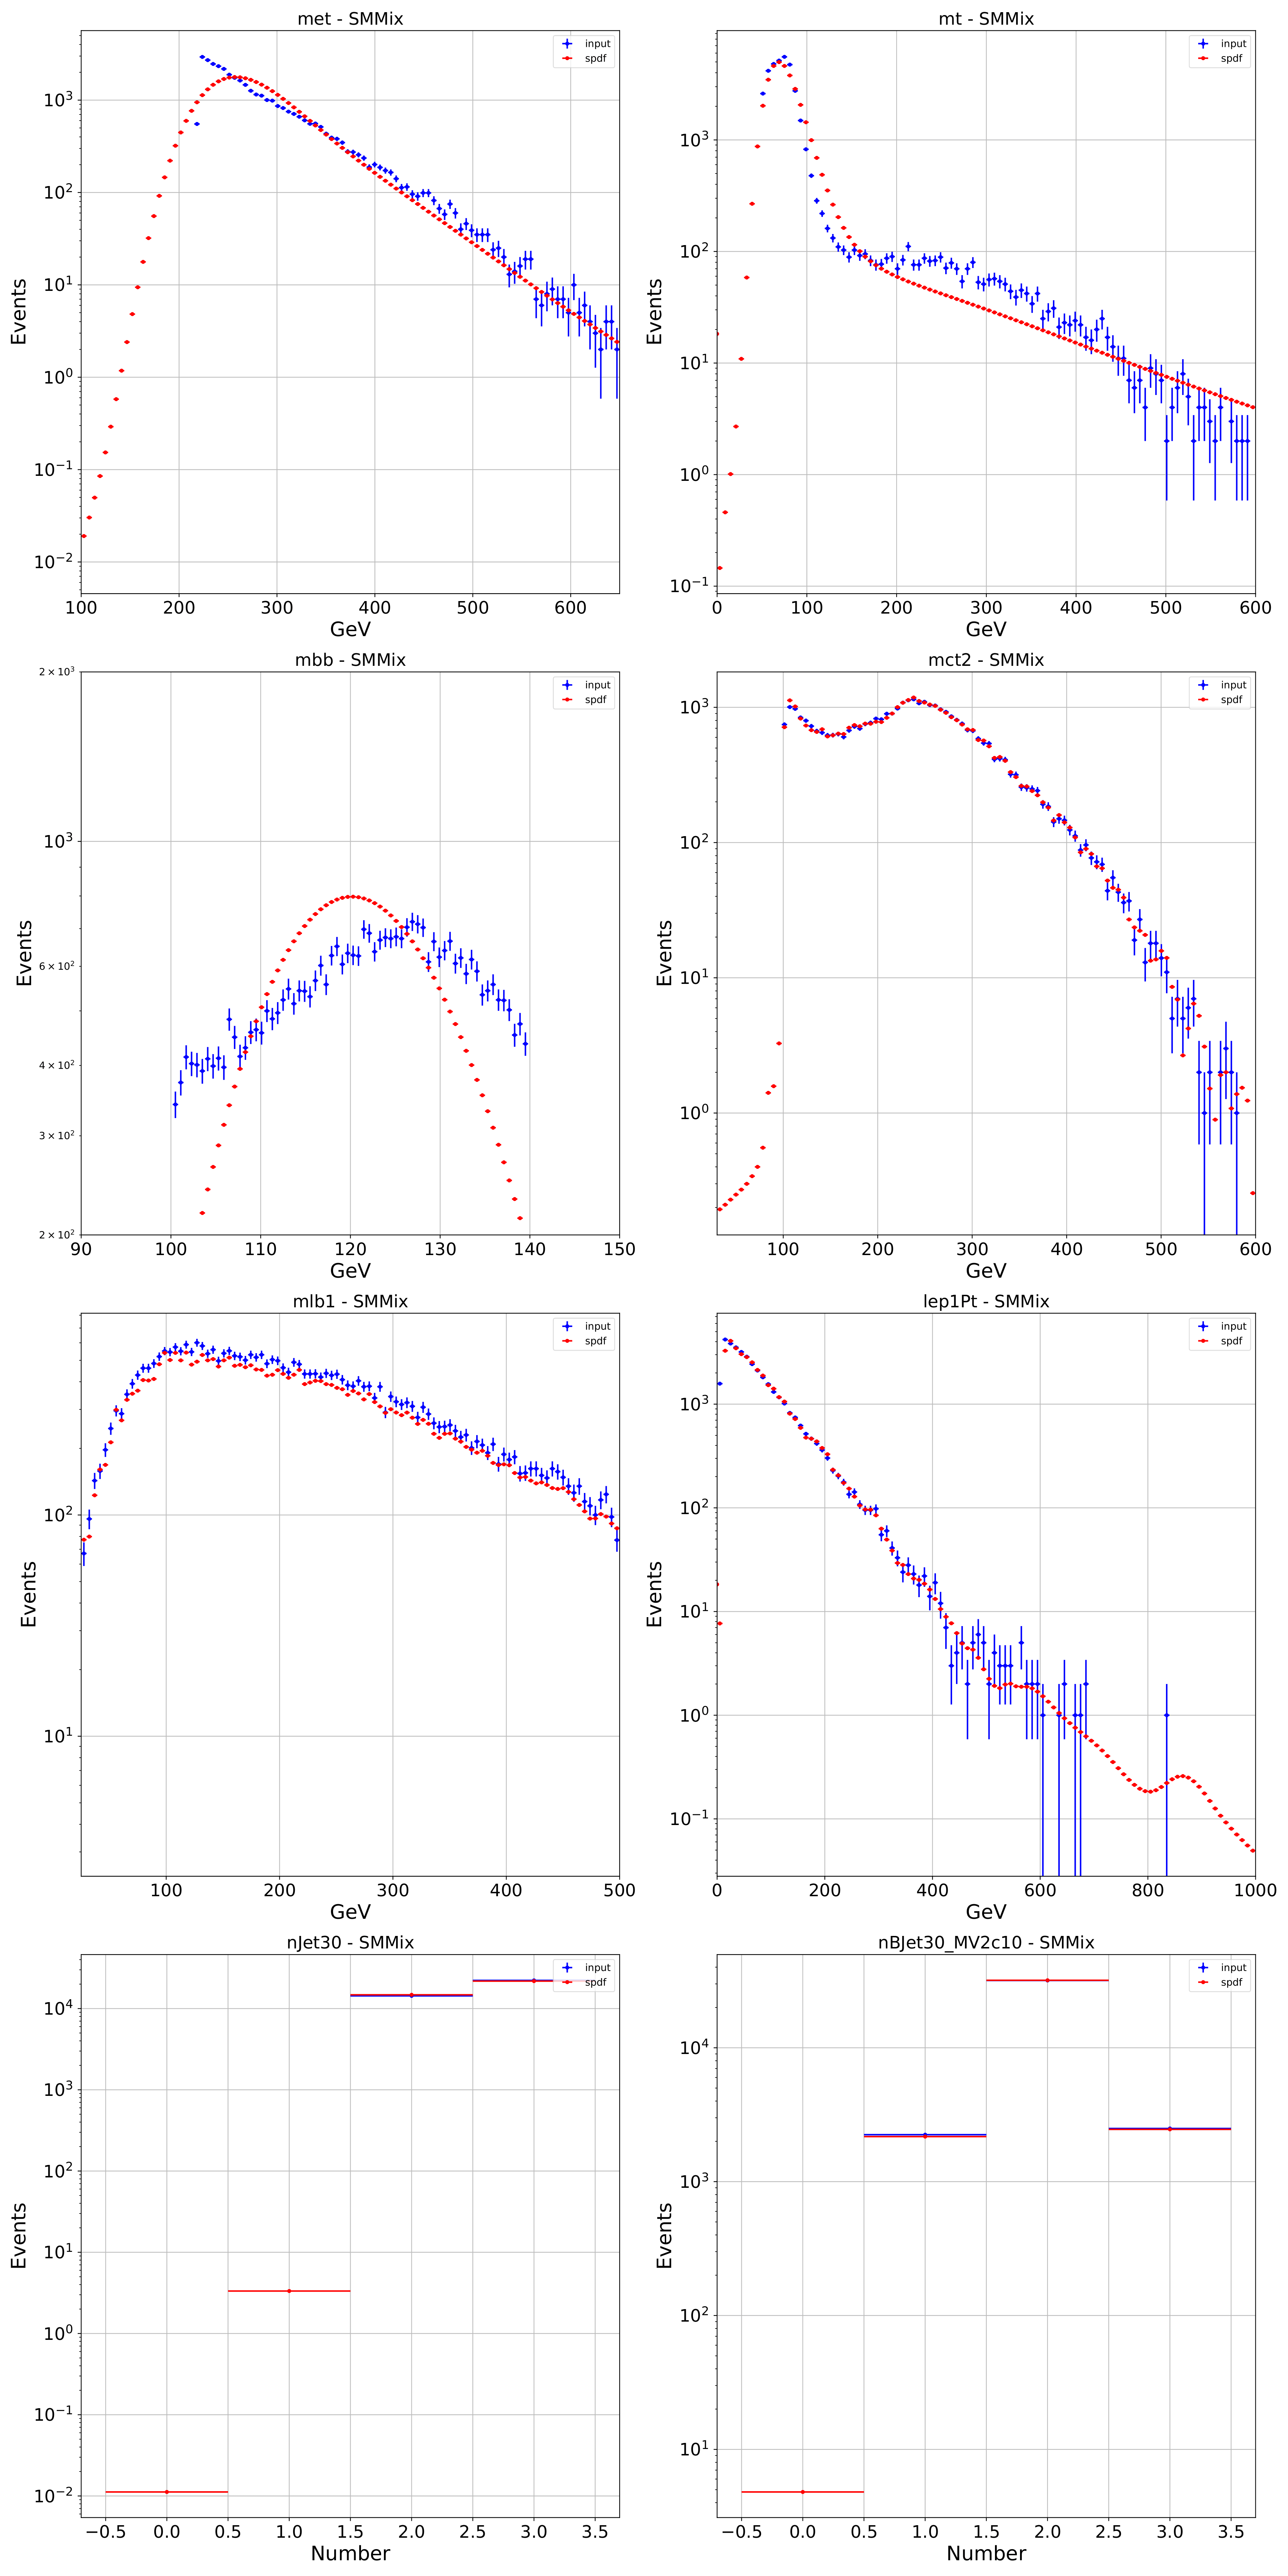
\includegraphics[width=0.56\textwidth]{figs/risultati_simulazione/ricostruzione.png}
	\caption{Confronto tra gli input in ingresso del VAE (in blu) e quelli ricostruiti (in rosso) per le otto componenti degli eventi di input relativi al background.}
	\label{ricostruzione}
\end{figure}

Dall'osservazione qualitativa della figura~\ref{ricostruzione} emerge che il processo di ricostruzione del VAE risulta piuttosto accurato per tutte le variabili ad eccezione della $\textit{mbb}$. \\
Tuttavia, come si vedrà più avanti, è possibile correggere questo risultato impostando un peso maggiore per tale variabile (ad esempio un peso pari a due o tre rispetto agli altri tutti pari ad uno). Inoltre, dopo aver constatato che è possibile indirizzare particolare attenzione sulla ricostruzione di specifiche variabili, si capirà come sfruttare questa situazione per ottenere un modello più sensibile ai vari tipi di segnale.\\

\color{red}
correzione da inserire: come si applica il peso e cosa rappresenta?
\color{black}

%%%%%%%%%%%%%%%%%%%%%%%%%%%%%%%%%%%%%%%%%%%%%%%%%%%%%%%%%%%%%%%%

\subsubsection{Distribuzione della loss di ricostruzione}
\label{reco_loss}

Per rendere un segnale riconoscibile è opportuno che il suo indice di anomalia lo contraddistingua rispetto a quello degli eventi di fondo. In questa tesi la misura adottata per discriminare tra fondo e segnale è l'errore di ricostruzione che il VAE commette durante la ricostruzione degli eventi. Altre scelte possibili sarebbero state quelle di utilizzare la loss totale data dalla somma della divergenza di Kullback-Lieber e della loss di ricostruzione oppure, al contrario, solo la divergenza di Kullback-Lieber. \\ 
Ad ogni modo, per ottenere l'errore di ricostruzione per ogni evento è sufficiente sommare quello sulle otto variabili. Da questi valori si ottiene quindi la distribuzione della $\textit{Loss}$, come quella riportata in figura \ref{distribuzione_loss}. 

\begin{figure}[h!]
	\centering
	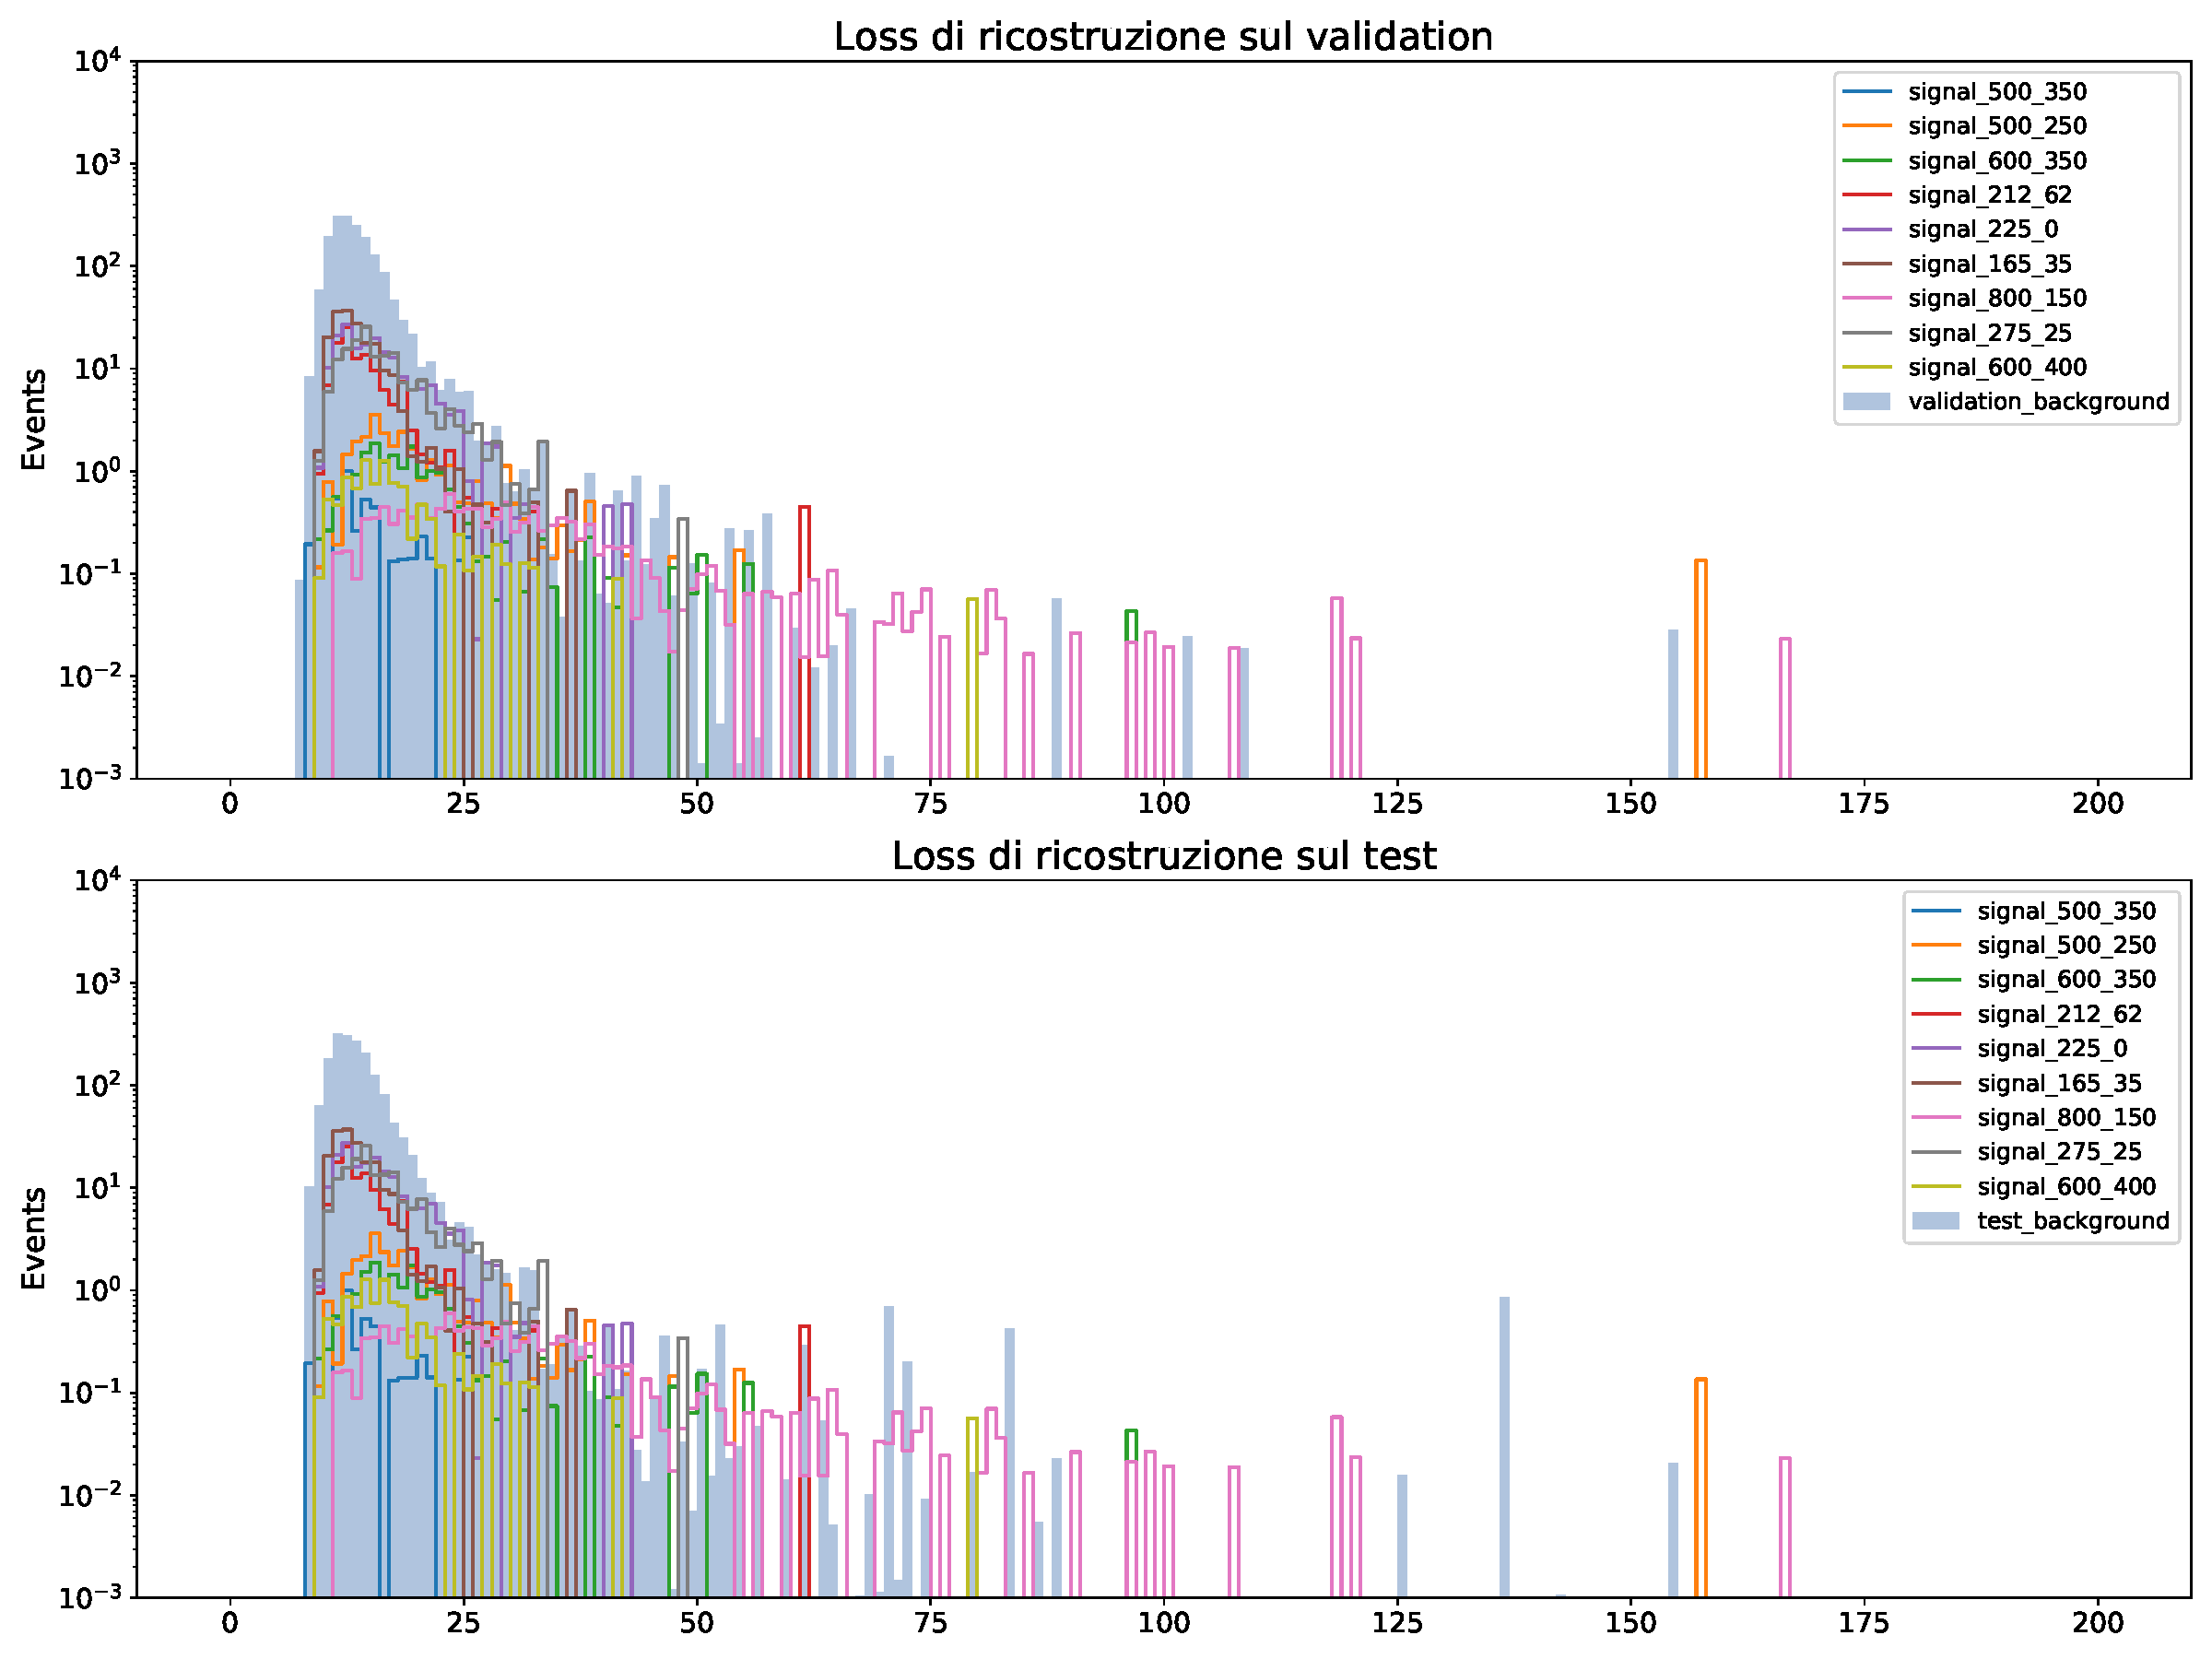
\includegraphics[width=0.85\textwidth]{figs/risultati_simulazione/distribuzioneLoss.pdf}
	\caption{Distribuzione della $\textit{Loss}$ per gli eventi di background e per quelli di segnale relativi ad alcune combinazioni delle masse di Chargino-Neutralino. La prima immagine è relativa al Vaidation data set, mentre la seconda al test data set.}
	\label{distribuzione_loss}
\end{figure}

In questa immagine, oltre alla distribuzione relativa agli eventi di background (istogramma blu) sia per il dataset di validation (sopra) che per quello di test (sotto), sono presenti anche le distribuzione relative ad alcune delle ipotesi di segnale (curve colorate) contraddistinte dalla diverse ipotesi sulle masse delle due particelle (chargino/neutralino). E' importante ricordare che le simulazioni MC degli eventi di segnale non sono mai state usate fino ad ora e solo in questa fase di test vengono date in input al modello. \\
Una situazione ideale prevede una distribuzione degli errori per gli eventi di fondo concentrata su valori della Loss inferiori rispetto alle analoghe distribuzioni relative agli eventi di segnale. In questo modo, infatti, la selezione del segnale risulta facilitata e il rapporto segnale/background aumenta.\\
Osservando le figure, una prima considerazione riguarda proprio questo aspetto. Infatti, la distribuzione della Loss per gli eventi di background presenta un picco spostato verso sinistra rispetto alle distribuzione relative agli eventi di segnale. Allo stesso tempo questa separazione non risulta molto netta, in particolare per alcuni tipi di segnale, caratterizzati da una struttura cinematica più simile a quella degli eventi di fondo. Per questo motivo si cercherà di trovare un modello che risulti più efficace in questo compito, sfruttando, ad esempio, una diversa pesatura delle variabili che caratterizzano un evento fisico.\\
Un altro aspetto non trascurabile e verificabile confrontando i due grafici della stessa figura \ref{distribuzione_loss}, riguarda l'\textbf{overfitting}. Infatti, giudicando la distribuzione degli eventi di background nei due grafici, si può vedere come la forma sia pressoché la stessa; questo permette di concludere che il modello è in grado di generalizzare, non adattandosi troppo al \textbf{validation data set} per poi essere in grado di generalizzare anche ad un set di dati mai visto prima (\textbf{test data set}).\\
Un'ultima osservazione può essere fatta pensando ad una possibile applicazione di questo algoritmo sui dati sperimentali, laddove la distinzione fra background e segnale non è nota a priori; infatti, osservando come le distribuzioni dei segnali si pongono rispetto a quella degli eventi di fondo e selezionando eventi con loss molto alta è possibile selezionare quelli più affini a processi di nuova fisica, e quindi fare un test di ipotesi su questi campioni selezionati.

\newpage

%%%%%%%%%%%%%%%%%%%%%%%%%%%%%%%%%%%%%%%%%%%%%%%%%%%%%%%%%%%%%%%%

\subsubsection{Esperimento di conteggio e regione di esclusione}
\label{esperimento di conteggio e regione di esclusione}

A questa prima analisi qualitativa ne viene fatta seguire una quantitativa, con la quale si vogliono definire per quali combinazioni delle masse delle due particelle il VAE riesce a discriminare, con una certa confidenza statistica, gli eventi di segnale da quelli di background. In questo modo sarà possibile delineare una regione di esclusione per i diversi segnali caratterizzati da diverse ipotesi circa le masse delle due particelle candidate.\\
Per portare a termine questo obiettivo si designa un esperimento di conteggio per confrontare l'ipotesi nulla, cioè di presenza di solo fondo nei dati, con quella alternativa che prevede invece anche la presenza del segnale. Nello specifico si procede in questo modo: dopo aver determinato il numero di eventi di fondo $N_b$ da selezionare, si ricava il valore di soglia della Loss relativa a questo numero. Successivamente, utilizzando lo stesso valore di soglia, si selezionano anche tutti gli eventi di segnale $N_s$ alla destra di tale valore per poi procedere all'esperimento di conteggio. In figura \ref{distribuzioneLossRiga} si riporta il caso in cui si vogliano selezionare 10 eventi SM. La soglia di selezione è quindi indicata dalla linea verticale della stessa immagine.

\begin{figure}[h!]
	\centering
	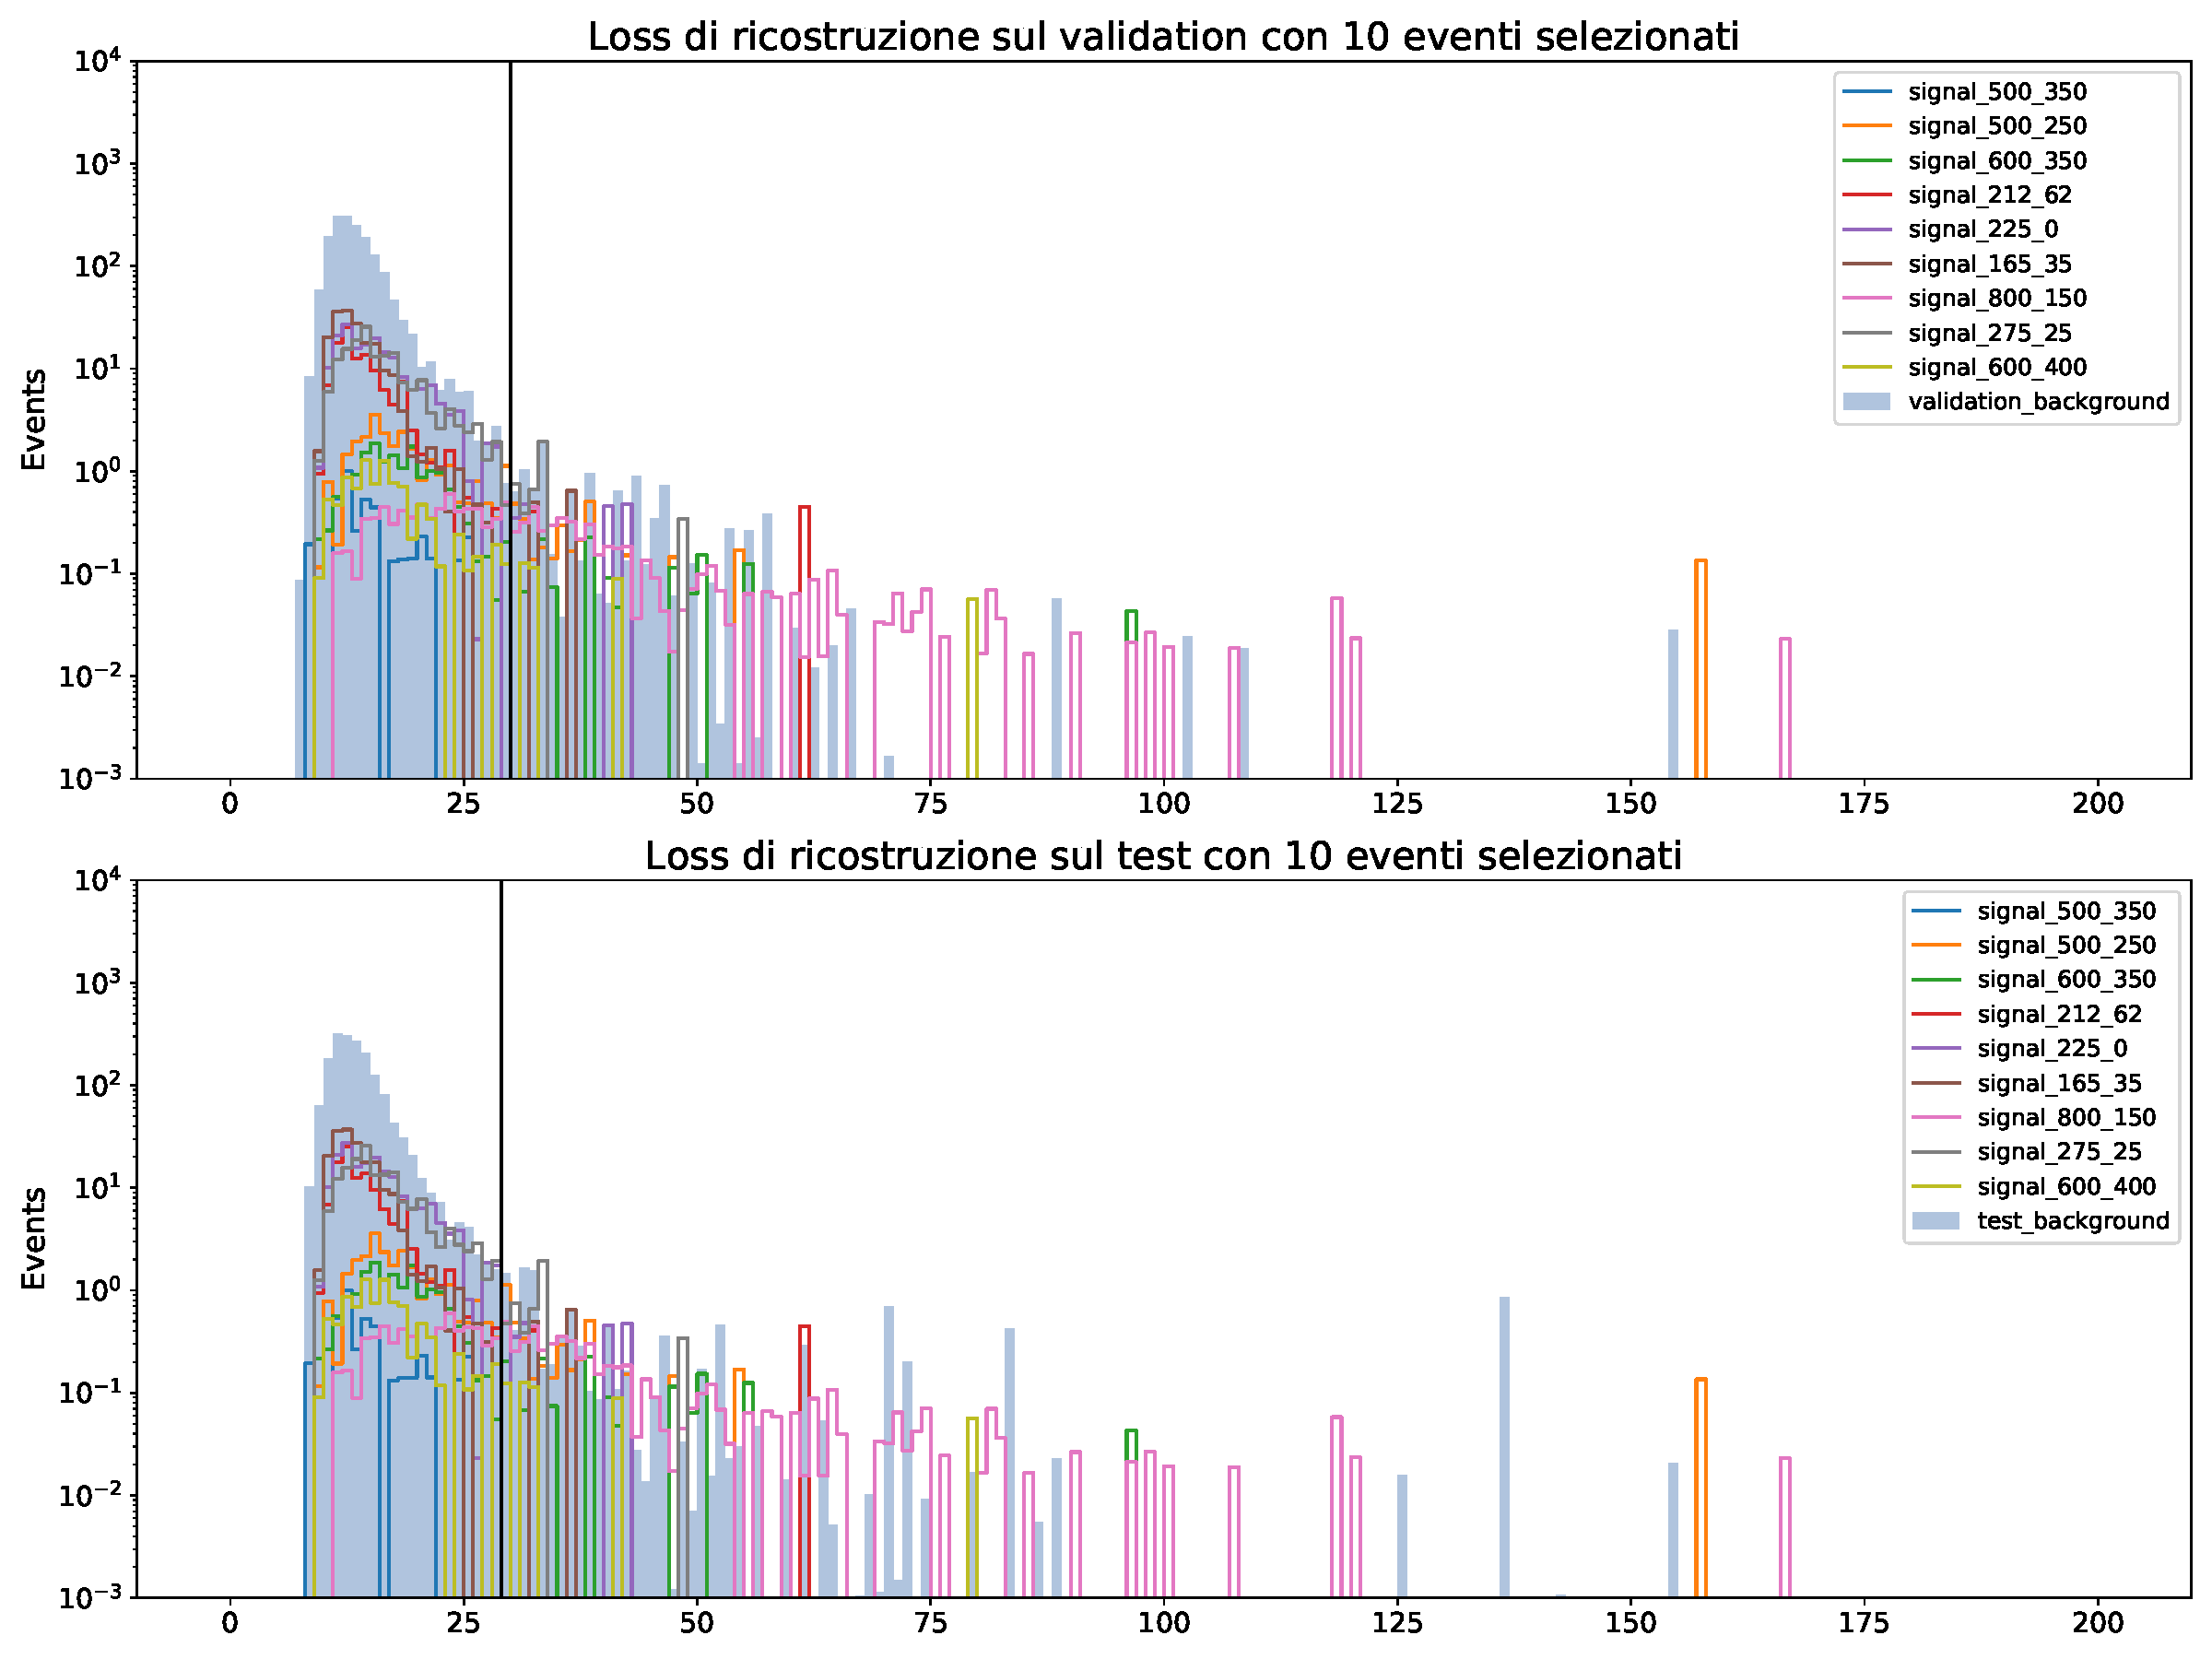
\includegraphics[width=0.99\textwidth]{figs/risultati_simulazione/distribuzioneLossRiga.pdf}
	\caption{Figura analoga all \ref{distribuzione_loss}, dove però la linea in nero mette in evidenza il processo di selezione degli eventi di background nella parte destra della distribuzione.}
	\label{distribuzioneLossRiga}
\end{figure}

Quindi, dopo aver ricavato $N_b$ ed $N_s$, si procede alla verifica dell'ipotesi nulla, ovvero la presenza di solo fondo nei dati; nello specifico si verifica che la probabilità di avere la somma $N_s + N_b$ di eventi sia compatibile con una distribuzione di Poisson centrata su di un valore pari a $N_b$ (in altre parole si calcola $p(N_b + N_s | N_b)$). Nel caso in cui tale probabilità sia inferiore al 5\%, si procede all'esclusione dell'ipotesi nulla in favore di quella alternativa di presenza di segnale nei dati.\\
Nelle figure~\ref{test-25-50-80} e~\ref{test-100-200-400} sono riportati i risultati dell'esperimento di conteggio e rappresentano la cosidetta regione di esclusione dove, lungo l'asse delle ascisse sono riportate le masse, considerate degeneri, delle due particelle prodotte nella collisione pp ($\chi^\pm_1$ e $\chi^0_2$), mentre lungo quello delle ordinate la massa della particella SUSY piu' leggera ($\chi^0_1$). Questi risultati sono riportati al variare del numero $N_{b}$ di eventi di fondo da selezionare per vedere se è in qualche modo possibile ottimizzare questo parametro in funzione della selezione del segnale. In altre parole si opera uno scan sui possibili valori $N_{b}$ che tornerà utile nella prossima sezione.\\
Tornando alla descrizione di queste immagini, si osservano sia punti rossi che verdi. I primi rappresentano le particolari combinazioni delle masse delle due particelle per le quali il VAE è in grado di discriminare fra segnale e background con sufficiente confidenza statistica, mentre i punti verdi indicano  quei segnali per cui tale discriminazione non può essere compiuta.\\
E' importante osservare come, aumentando il numero di eventi da selezionare nella zona di ipotesi con basse masse ($m < 300 GeV$), si evidenzia un incremento della sensibilità al segnale; l'opposto avviene invece per le zone con $m > 600 GeV$, mentre per la zona intermedia un buon risultato sembra emergere nel range $50 GeV - 80 GeV$ eventi di fondo da selezionare. Questo è dovuto al fatto che la sezione d'urto attesa per la produzione delle particelle SUSY diminuisce lungo l'asse delle ascisse. Questo fa si che il campione statistico del segnale sia più grande a basse masse e più piccolo a masse più alte. In questo modo la selezione deve essere maggiormente stringente al crescere della massa così da ottenere un campione adeguato per il test di ipotesi.\\
In ogni caso scegliendo tre selezioni diverse, una per regione, è possibile designare un'unica regione di esclusione avendo ottimizzato la procedura nelle diverse regioni di massa. E' giusto rimarcare anche come questo scan sia stato condotto su dati di validation in quanto relativo ad un processo di ottimizzazione degli iperparametri e quindi riconducibile ad un fine-tuning del modello. Come tale non può essere condotto sugli stessi dati di test su cui i risultati finali verrano estratti. Infatti, solo i risultati finali della prossima sezione prendono in considerazione il test set per evitare possibili bias sugli esiti finali.

\color{red}
commento vuoto \\
chiedere chiarimento sull'ultimo commento.\\
\color{black}

\newpage

\begin{figure}[h!]
	\centering
	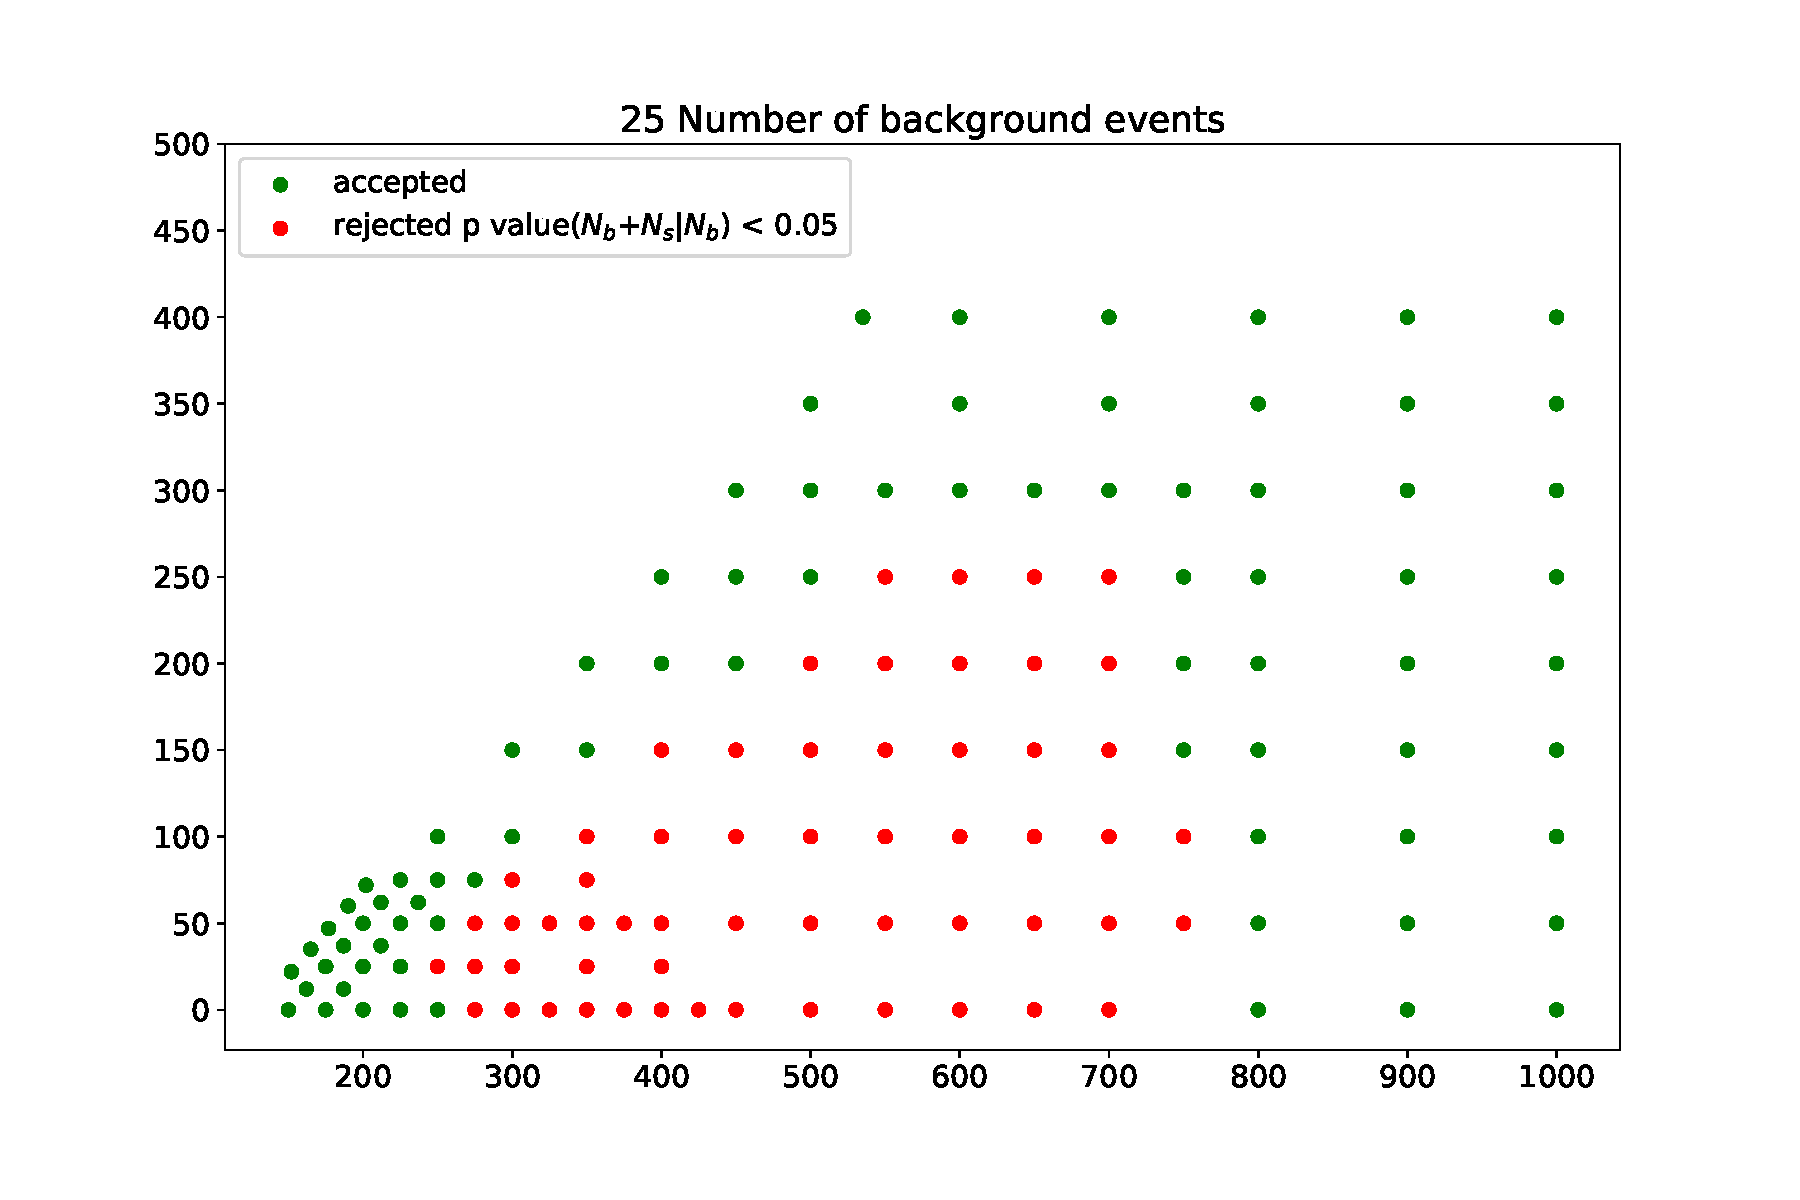
\includegraphics[width=0.72\textwidth]{figs/risultati_simulazione/25.pdf}
	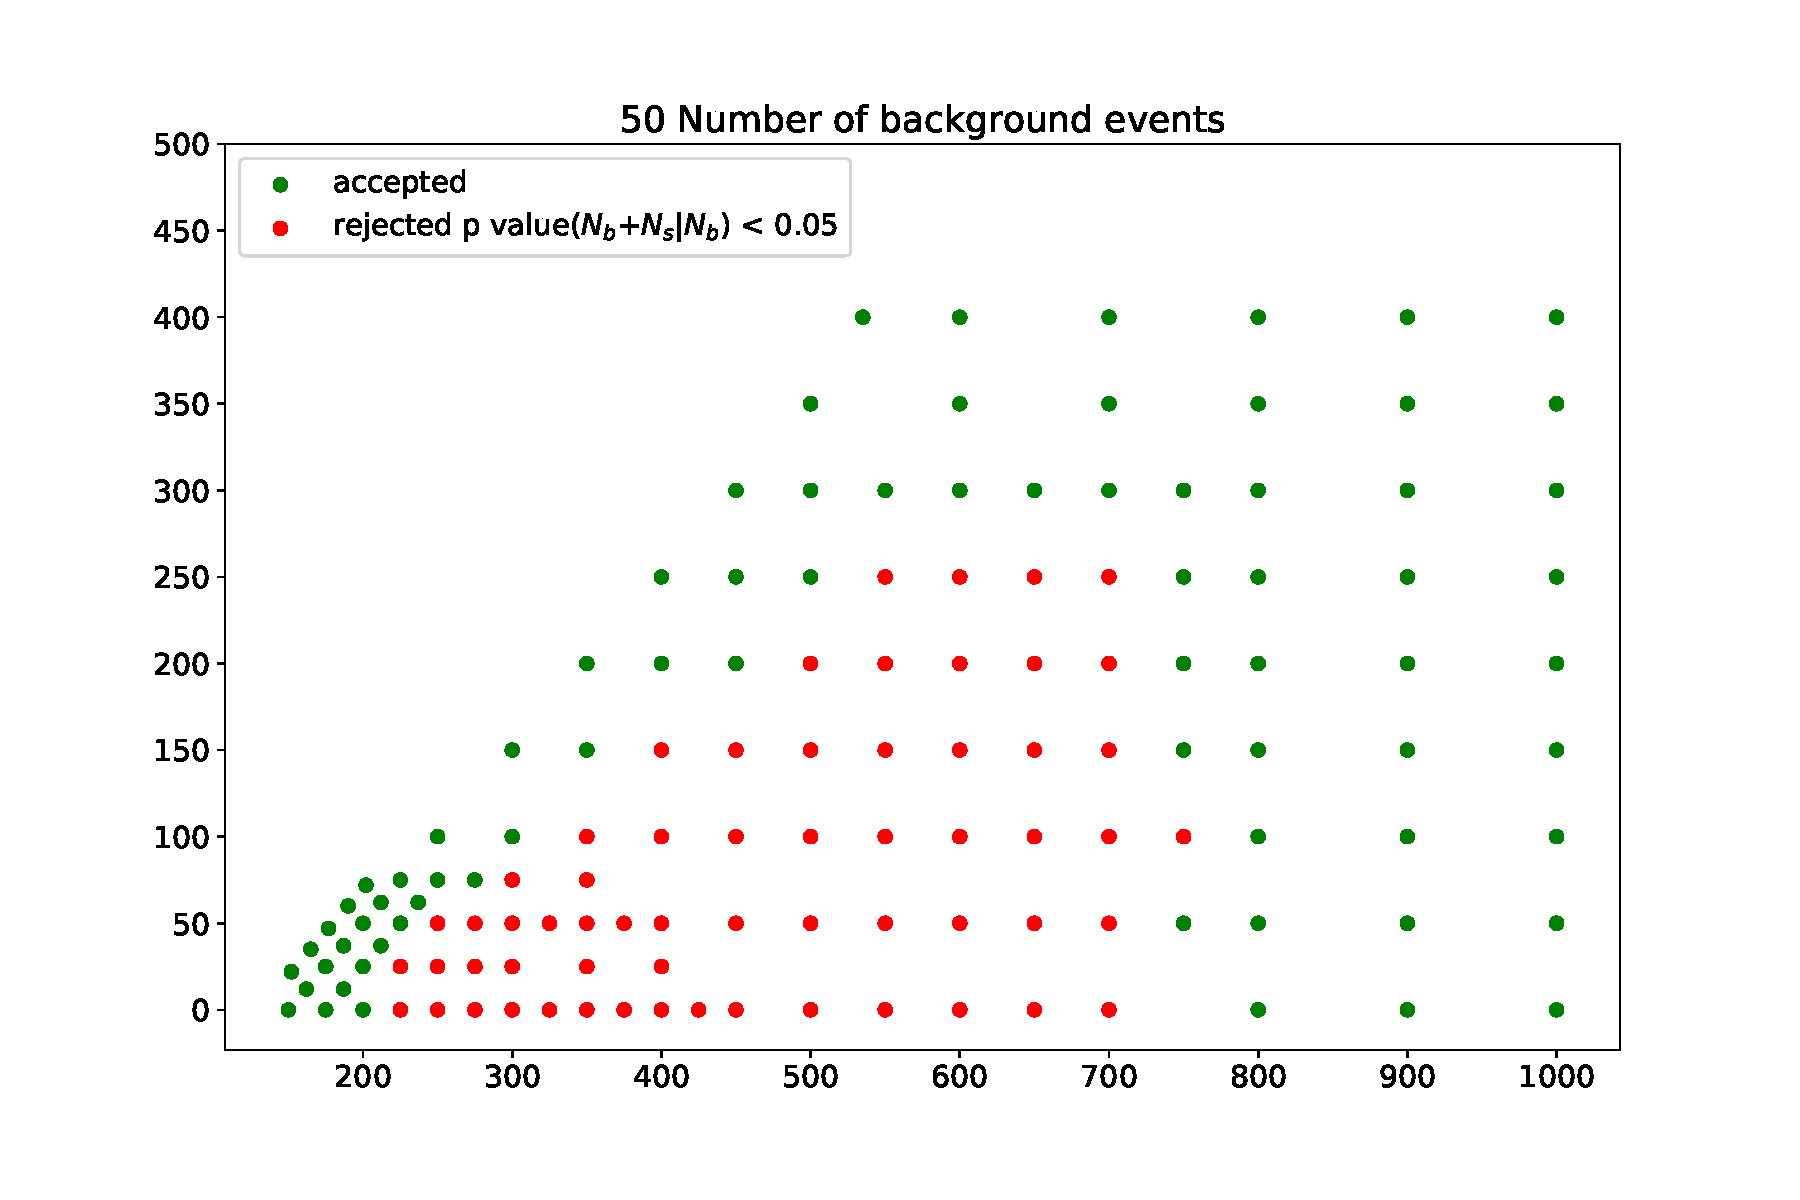
\includegraphics[width=0.72\textwidth]{figs/risultati_simulazione/50.pdf}
	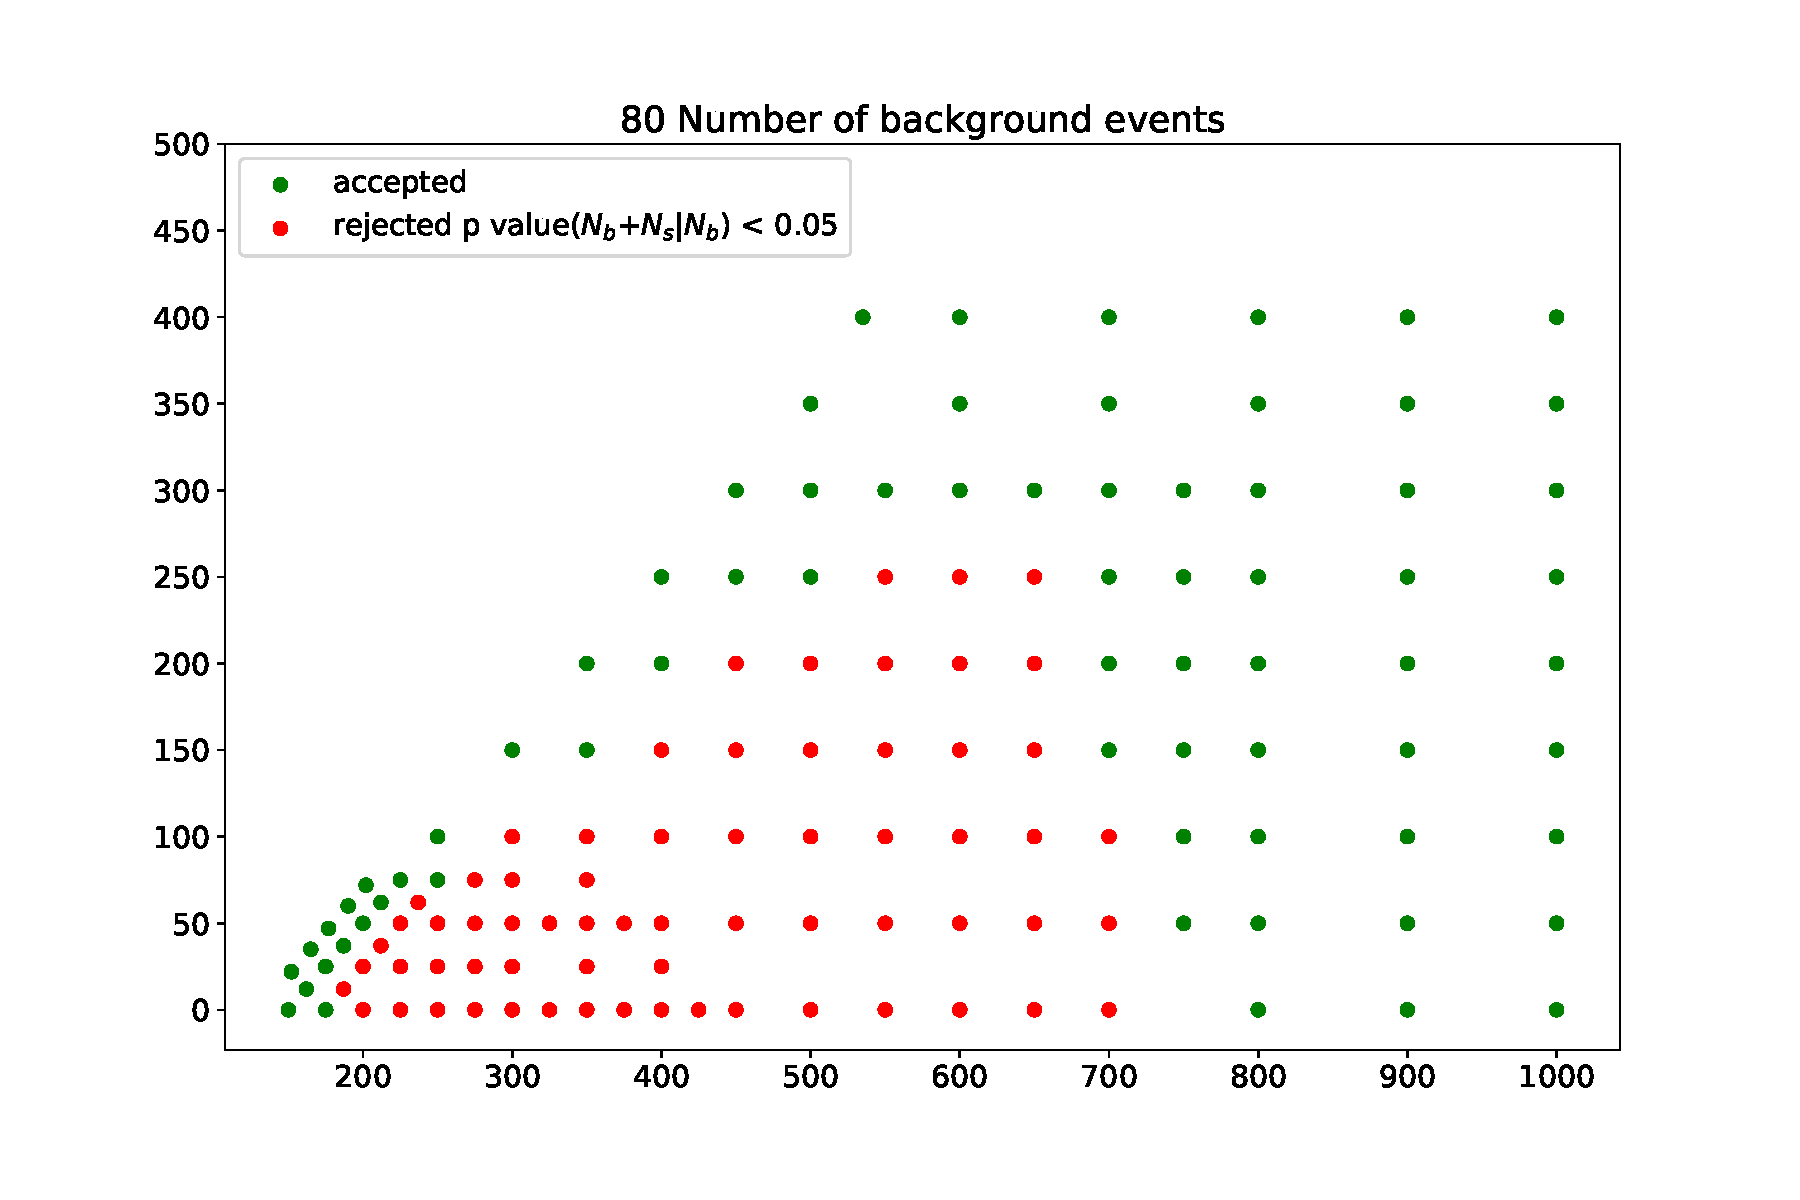
\includegraphics[width=0.72\textwidth]{figs/risultati_simulazione/80.pdf}
	\caption{Risultati degli esperimenti di conteggio per, rispettivamente, 25, 50 e 80 eventi di background selezionati nella parte destra della distribuzione della Loss.}
	\label{test-25-50-80}
\end{figure}
\begin{figure}[h!]
	\centering
	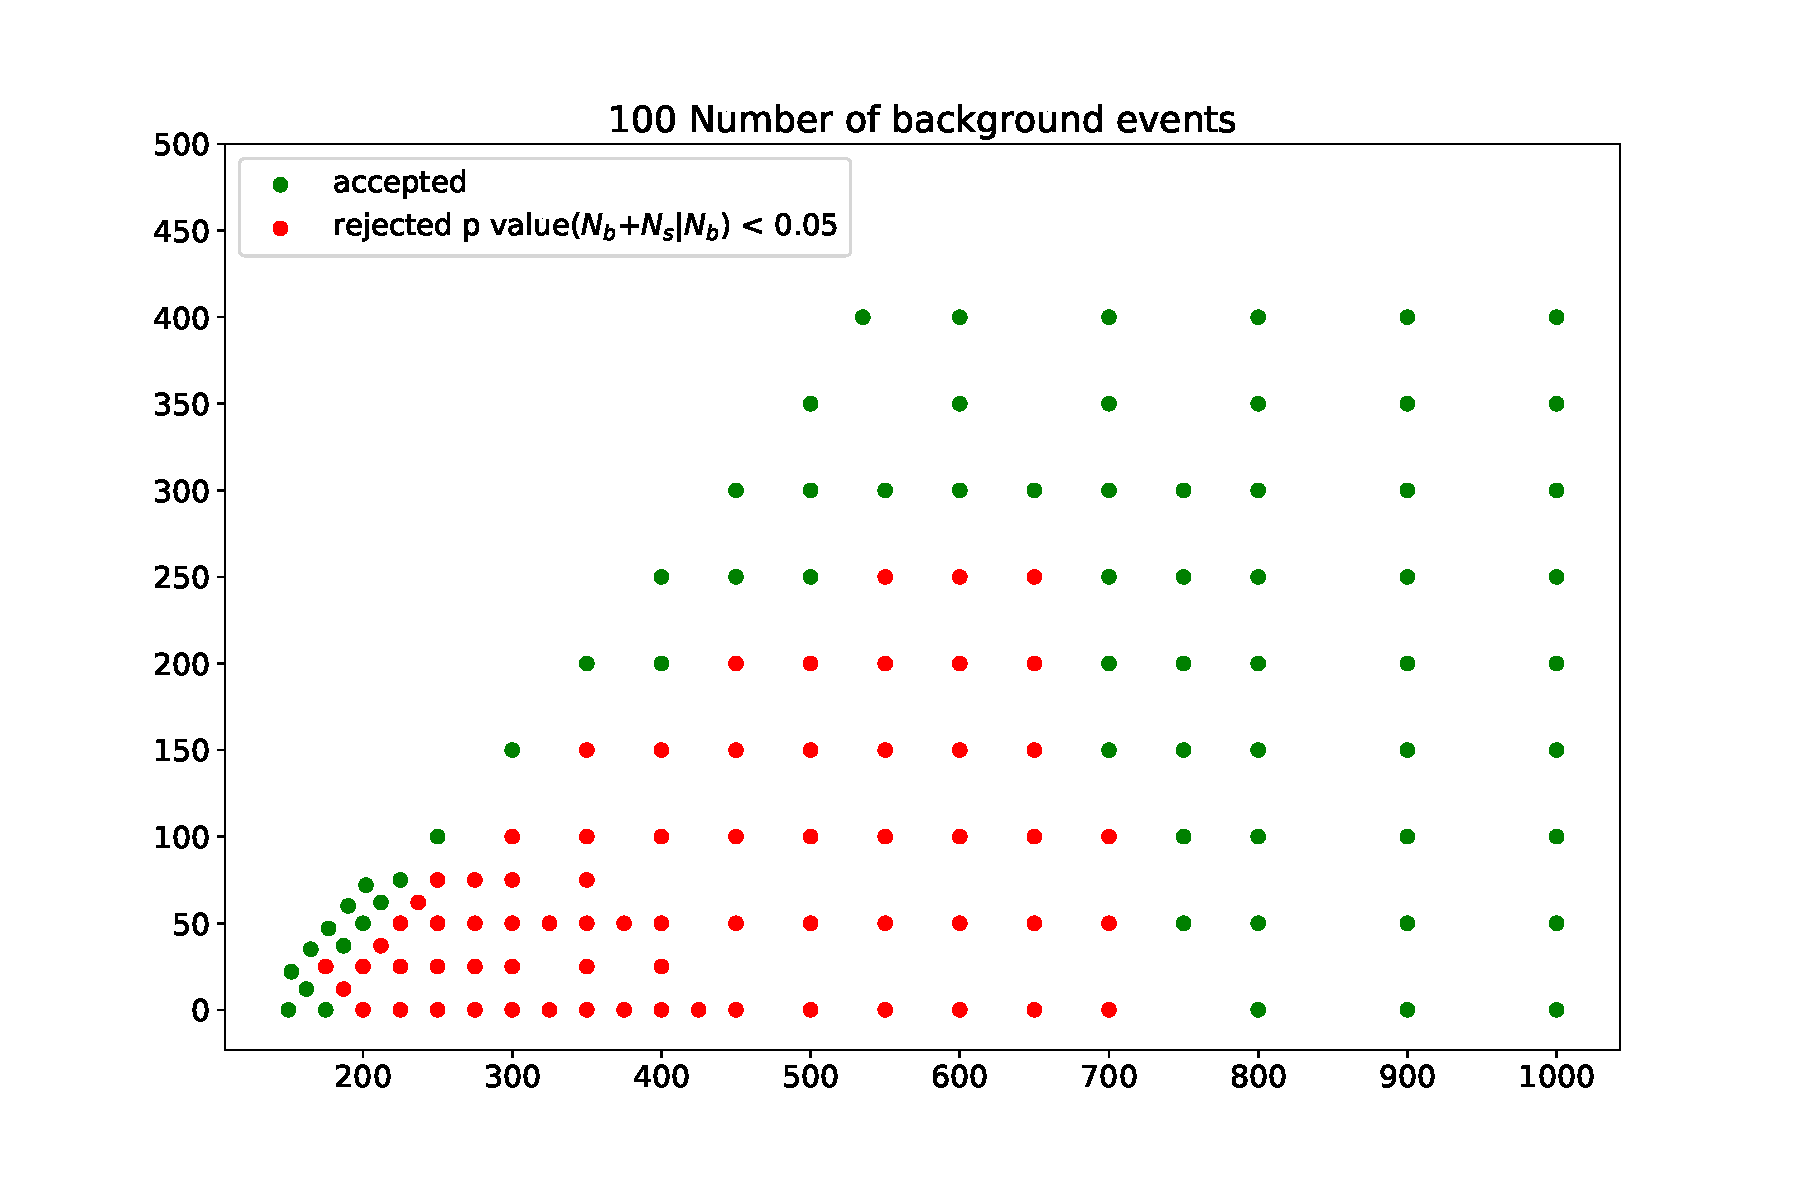
\includegraphics[width=0.71\textwidth]{figs/risultati_simulazione/100.pdf}
	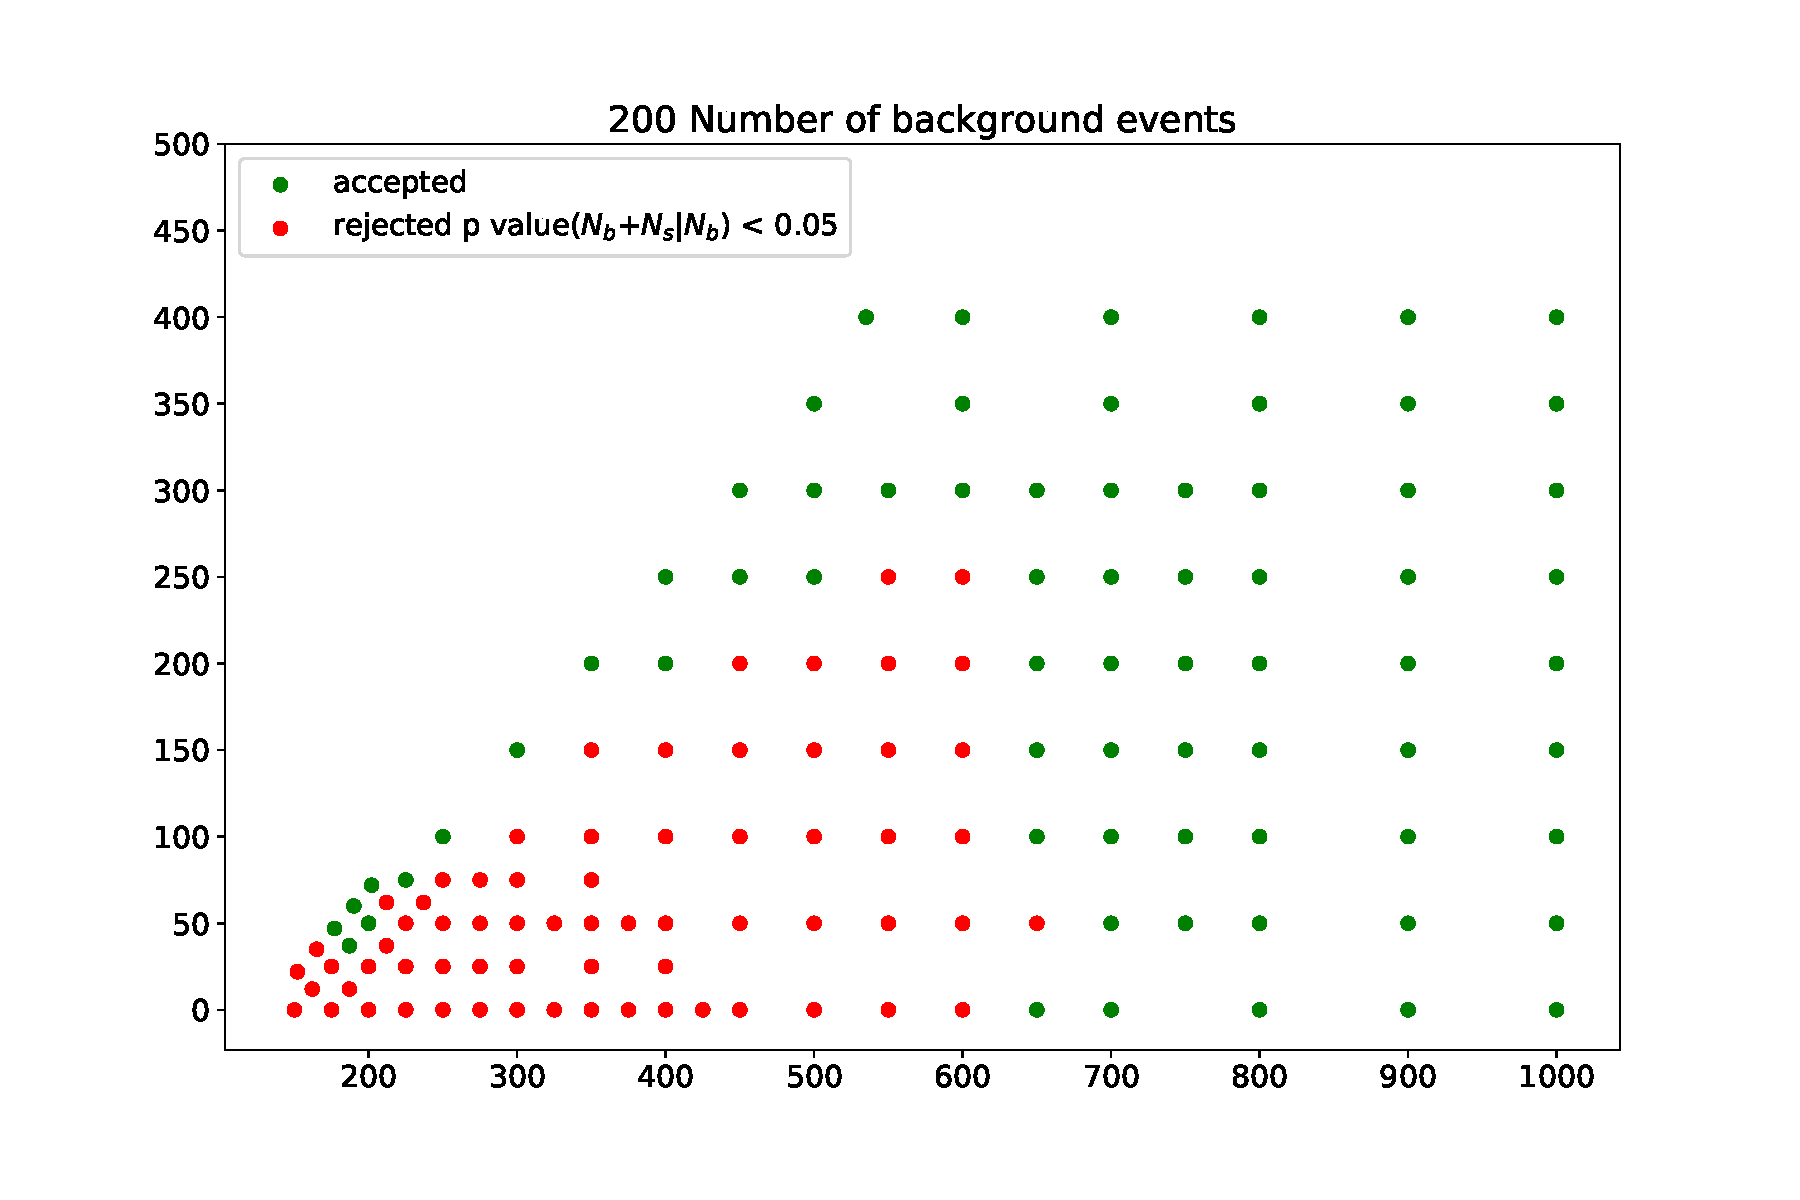
\includegraphics[width=0.71\textwidth]{figs/risultati_simulazione/200.pdf}
	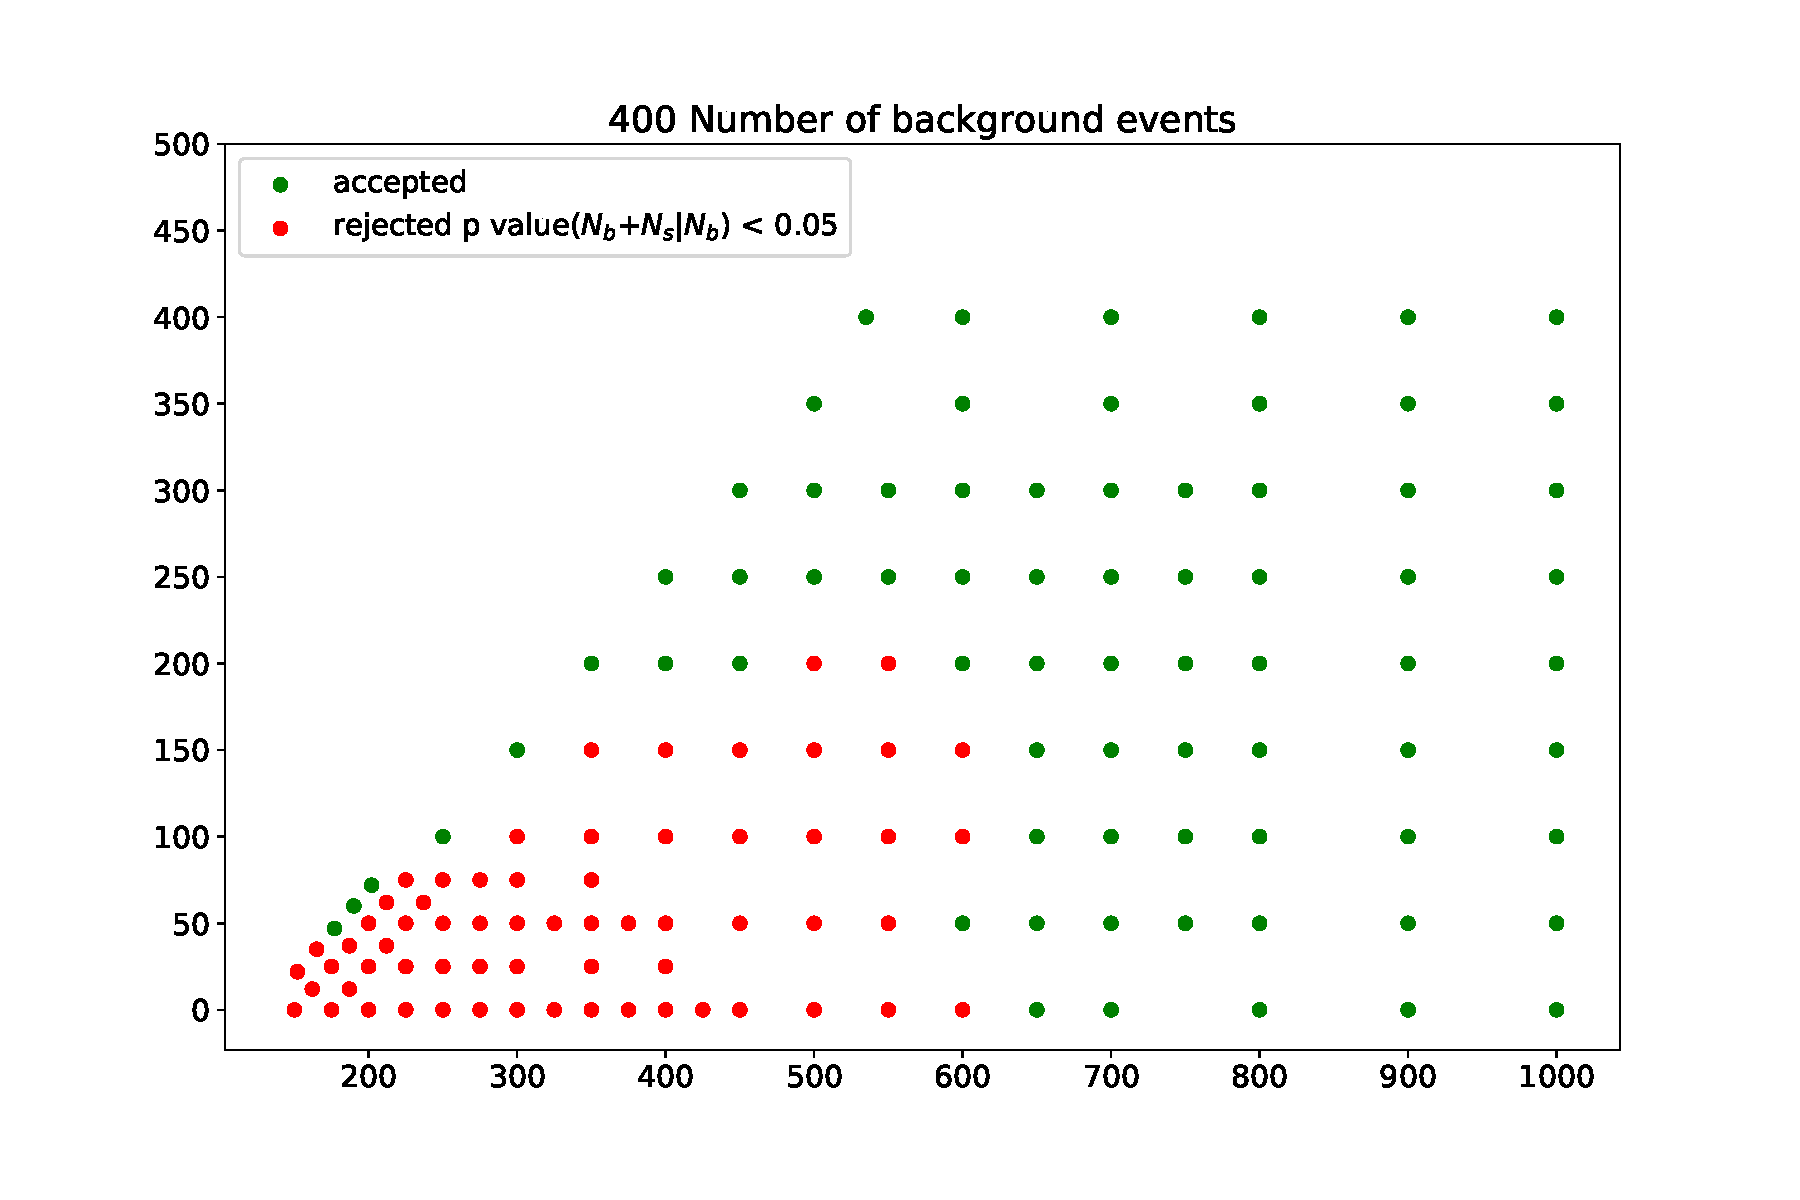
\includegraphics[width=0.71\textwidth]{figs/risultati_simulazione/400.pdf}
	\caption{Risultati degli esperimenti di conteggio per, rispettivamente, 100, 200 e 400 eventi di background selezionati nella parte destra della distribuzione della Loss.}
	\label{test-100-200-400}
\end{figure}


%%%%%%%%%%%%%%%%%%%%%%%%%%%%%%%%%%%%%%%%%%%%%%%%%%%%%%%%%%%%%%%%

\subsubsection{Regione di esclusione ottimizzata}
\label{regione di esclusione}


A questo punto dopo aver individuato le tre zone lungo l'asse delle ascisse, rispettivamente per valori $ m(chi^\pm_1/chi^0_2) \le 300 GeV$ , $300 GeV < m \le 600 GeV$ e $m > 600 GeV$, è necessario ricavare il numero ottimale di eventi di background da selezionare in modo da ottimizzare la sensibilità agli eventi di segnale. Da un semplice conteggio dei punti evidenziati in rosso si ottiene che la combinazione ottimale prevede di selezionare 400 eventi di background per la prima zona, 100 per la seconda e 25 per la terza. In figura~\ref{mix} viene riportato l'esito finale dell'esperimento, selezionando per ognuna delle tre zone il valore ottimale di eventi di background da selezionare.

\begin{figure}[h!]
	\centering
	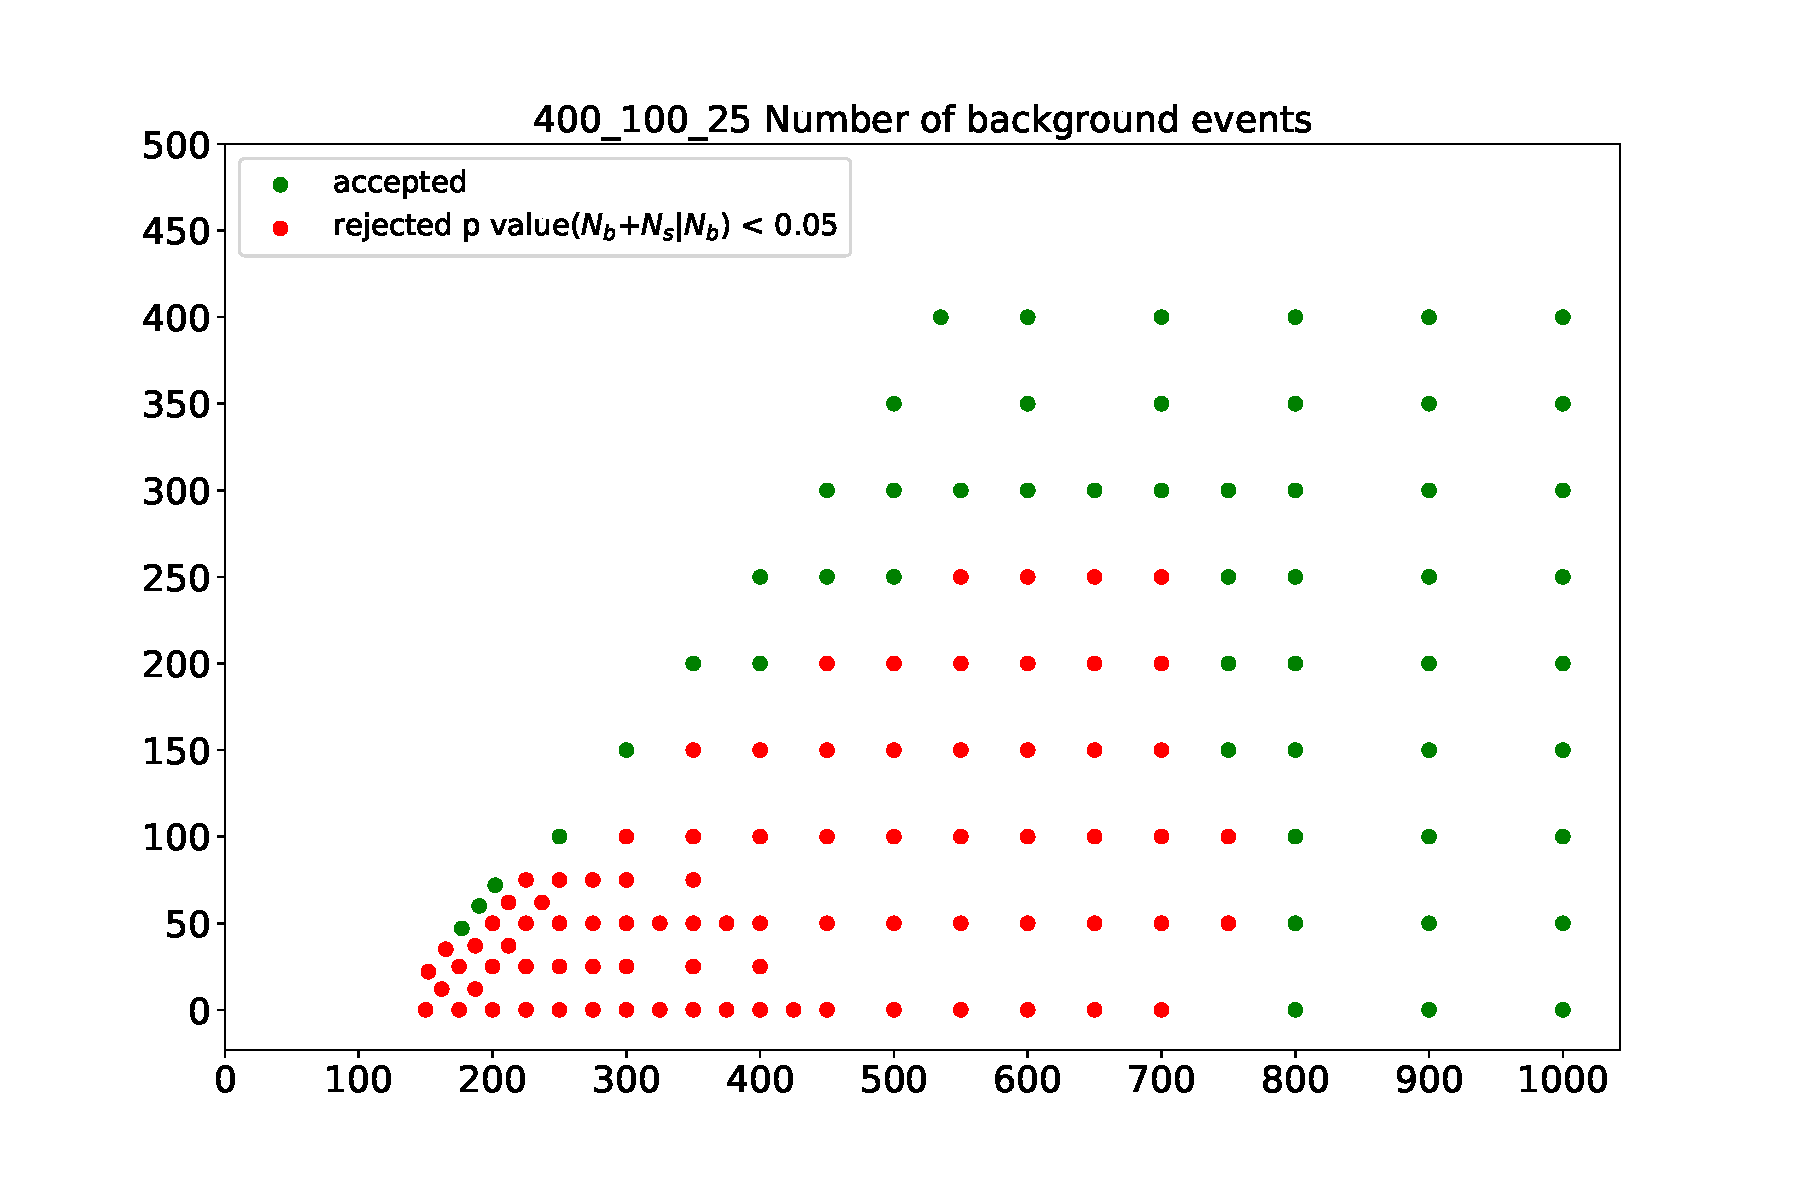
\includegraphics[width=0.90\textwidth]{figs/risultati_simulazione/mix.pdf}
	\caption{Risultato del processo di ottimizzazione nella distinzione fra background e segnale. Sono stati utilizzati i risultati ottimali in ciascuna delle tre zone individuate.}
	\label{mix}
\end{figure}

Questa ottimizzazione consente di raggiungere delle sensibilità al segnale SUSY analoghe a quella dei metodi \textbf{cut and count} [metti figura per il confronto]
Rimangono pero' alcune questioni aperte, legate alla cattiva ricostruzione della variabile mbb, e se ci siano variabili più sensibili delle altre tra quelle utilizzate nella presente analisi.

\color{red}
figura per il confronto??
\color{black}

\newpage

\subsubsection{Effetti della variazione dei pesi sulle variabili fisiche nel processo di apprendimento}
\label{effetti variazione pesi}

Per ottimizzare ulteriormente la selezione è possibile operare sugli iperparametri del VAE. In particolare si vuole vedere in che modo cambia la sensibilità del modello agli eventi di segnale cambiando i pesi relativi alle diverse variabili che costituiscono un evento fisico.\\
Nella precedente ottimizzazione la rigenerazione di una delle variabili ($\textit{mbb}$) non è stata soddisfacente. Per questo motivo si è provato ad impostare un peso maggiore per questa variabile ed il risultato è riportato in figura~\ref{mbb_ottimizzazione} (nello specifico è stato scelto un peso pari a tre per la variabile $\textit{mbb}$ e ad uno per le altre).

\begin{figure}[h!]
	\centering
	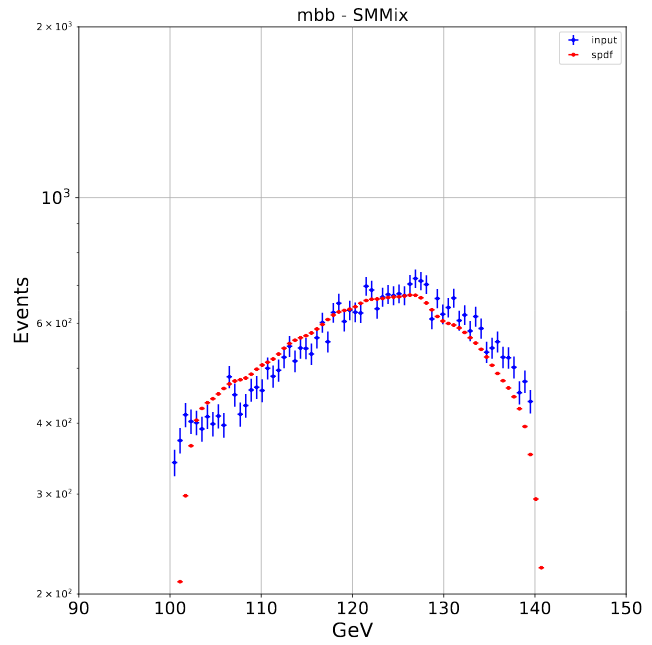
\includegraphics[width=0.65\textwidth]{figs/risultati_simulazione/verifica_mbb.png}
	\caption{Esito del processo di ricostruzione della variabile $\textit{mbb}$ dopo aver impostato un peso pari a tre per tale variabile e mantenendo quelli delle altre variabili pari ad uno. In blu sono riportati i dati originali ed in rosso quelli ricostruiti.}
	\label{mbb_ottimizzazione}
\end{figure}

Risulta evidente che questo piccolo accorgimento in fase di simulazione ha permesso di ottenere un'ottima ricostruzione della variabile $\textit{mbb}$, mantenendo inalterata la qualità delle altre. Ciò è avvenuto perché, aumentando il peso su tale variabile, aumenta anche il relativo errore nella ricostruzione (l'errore viene moltiplicato per il peso); di conseguenza l'algoritmo, operando la minimizzazione della \textbf{loss} totale, viene forzato ad occuparsi maggiormente della ricostruzione della variabile $\textit{mbb}$. \\
Questo spunto suggerisce che è effettivamente possibile condizionare il modello sulla ricostruzione delle diverse variabili, di conseguenza ci si chiede se vincolando l'algoritmo su alcune grandezze fisiche particolari sia possibile ottenere un processo di discriminazione migliore.

\newpage

Si passa quindi a verificare se nel processo di classificazione in segnale e background vi siano alcune variabili più discriminanti di altre; per far emergere ciò bisogna assegnare pesi diversi alle diverse variabili e osservare il conseguente risultato: emerge che ci sono effettivamente tre variabili più discriminanti delle altre, cioè $\textit{met}$, $\textit{mt}$ e $\textit{mct2}$). Nello specifico sono stati assegnati i pesi rispettivamente pari a 5,10,10 a queste tre variabili ed il risultato finale ottenuto è stato riportato in figura~\ref{mix_ottimizzato}, per poter essere confrontato con il risultato in figura~\ref{mix} dove i pesi erano tutti pari ad uno.

\begin{figure}[h!]
	\centering
	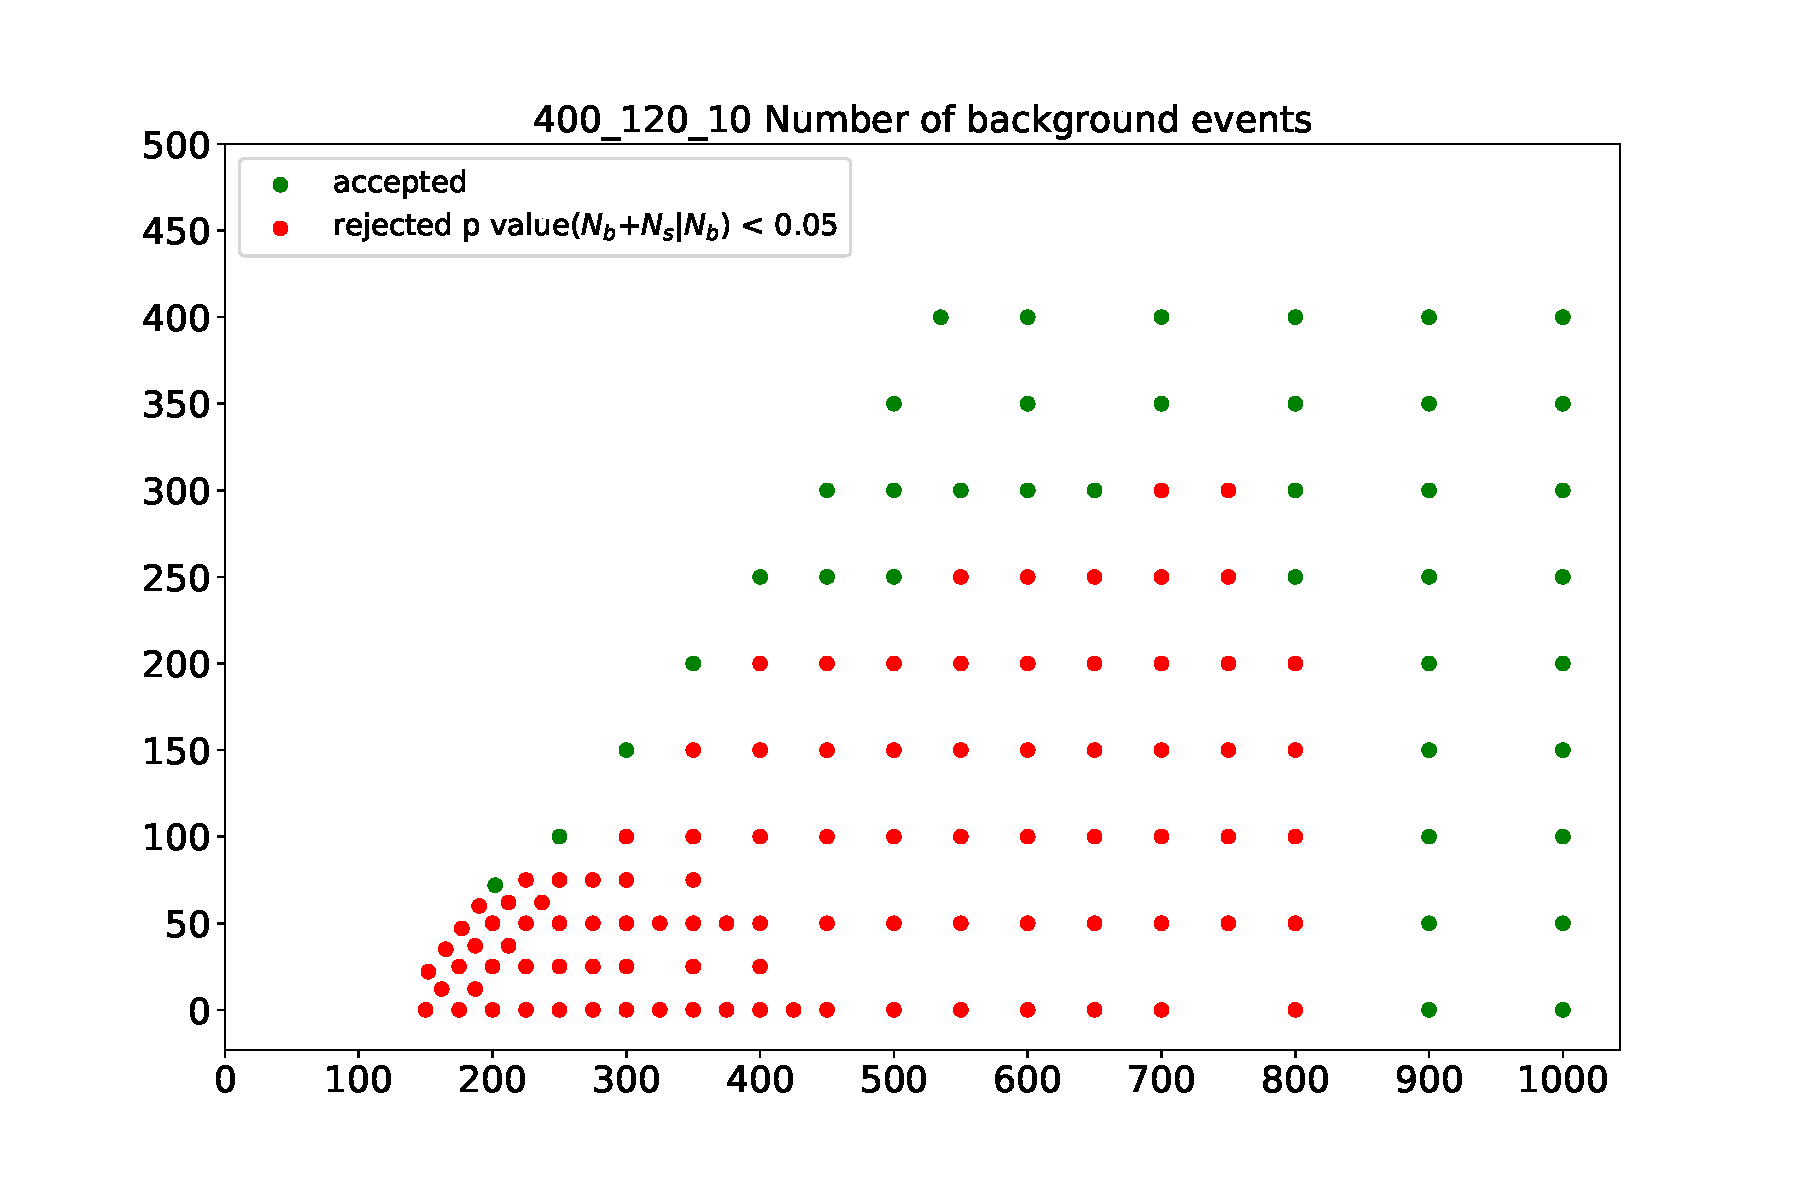
\includegraphics[width=0.90\textwidth]{figs/risultati_simulazione/mix_ottimizzato.pdf}
	\caption{Risultato analogo a quello riportato in figura~\ref{mix}, ma utilizzando pesi differenti per le variabili più discriminanti.}
	\label{mix_ottimizzato}
\end{figure}

Emerge dal confronto fra le due figure che quest'ultima configurazione di iperparametri permette la distinzione del segnale di background per un numero maggiore di possibili combinazioni delle masse delle due particelle. Nel primo caso con pesi tutti pari ad uno il numero totale di combinazioni delle masse delle particelle e quindi di modelli è 82, mentre in questo secondo caso si arriva a quota 96. \\
Quindi si giunge alla conclusione che, in questo caso specifico, pesare in maniere differente le variabili che costituiscono gli eventi permette di ottenere una sensibilità maggiore, ovvero il VAE riesce ad essere discriminante per un maggior numero di possibili eventi di segnale.

